% A LaTeX template for MSc Thesis submissions to 
% Politecnico di Milano (PoliMi) - School of Industrial and Information Engineering
%
% S. Bonetti, A. Gruttadauria, G. Mescolini, A. Zingaro
% e-mail: template-tesi-ingind@polimi.it
%
% Last Revision: October 2021
%
% Copyright 2021 Politecnico di Milano, Italy. NC-BY

\documentclass{Configuration_Files/PoliMi3i_thesis}

%------------------------------------------------------------------------------
%	REQUIRED PACKAGES AND  CONFIGURATIONS
%------------------------------------------------------------------------------

% CONFIGURATIONS
\usepackage{parskip} % For paragraph layout
\usepackage{setspace} % For using single or double spacing
\usepackage{emptypage} % To insert empty pages
\usepackage{multicol} % To write in multiple columns (executive summary)
\setlength\columnsep{15pt} % Column separation in executive summary
\setlength\parindent{0pt} % Indentation
\raggedbottom  

% PACKAGES FOR TITLES
\usepackage{titlesec}
% \titlespacing{\section}{left spacing}{before spacing}{after spacing}
\titlespacing{\section}{0pt}{3.3ex}{2ex}
\titlespacing{\subsection}{0pt}{3.3ex}{1.65ex}
\titlespacing{\subsubsection}{0pt}{3.3ex}{1ex}
\usepackage{color}

% PACKAGES FOR LANGUAGE AND FONT
\usepackage[english]{babel} % The document is in English  
\usepackage[utf8]{inputenc} % UTF8 encoding
\usepackage[T1]{fontenc} % Font encoding
\usepackage[11pt]{moresize} % Big fonts

% PACKAGES FOR IMAGES
\usepackage{graphicx}
\usepackage{transparent} % Enables transparent images
\usepackage{eso-pic} % For the background picture on the title page
\usepackage{subfig} % Numbered and caption subfigures using \subfloat.
\usepackage{tikz} % A package for high-quality hand-made figures.
\usetikzlibrary{}
\graphicspath{{./Images/}} % Directory of the images
\usepackage{caption} % Coloured captions
\usepackage{xcolor} % Coloured captions
\usepackage{amsthm,thmtools,xcolor} % Coloured "Theorem"
\usepackage{float}

% STANDARD MATH PACKAGES
\usepackage{amsmath}
\usepackage{amsthm}
\usepackage{amssymb}
\usepackage{amsfonts}
\usepackage{bm}
\usepackage[overload]{empheq} % For braced-style systems of equations.
\usepackage{fix-cm} % To override original LaTeX restrictions on sizes

% PACKAGES FOR TABLES
\usepackage{tabularx}
\usepackage{longtable} % Tables that can span several pages
\usepackage{colortbl}

% PACKAGES FOR ALGORITHMS (PSEUDO-CODE)
\usepackage{algorithm}
\usepackage{algorithmic}

% PACKAGES FOR REFERENCES & BIBLIOGRAPHY
\usepackage[colorlinks=true,linkcolor=black,anchorcolor=black,citecolor=black,filecolor=black,menucolor=black,runcolor=black,urlcolor=black]{hyperref} % Adds clickable links at references
\usepackage{cleveref}
\usepackage[square, numbers, sort&compress]{natbib} % Square brackets, citing references with numbers, citations sorted by appearance in the text and compressed
\bibliographystyle{abbrvnat} % You may use a different style adapted to your field

% OTHER PACKAGES
\usepackage{pdfpages} % To include a pdf file
\usepackage{afterpage}
\usepackage{lipsum} % DUMMY PACKAGE
\usepackage{fancyhdr} % For the headers
\fancyhf{}

% Input of configuration file. Do not change config.tex file unless you really know what you are doing. 
% Define blue color typical of polimi
\definecolor{bluepoli}{cmyk}{0.4,0.1,0,0.4}

% Custom theorem environments
\declaretheoremstyle[
  headfont=\color{bluepoli}\normalfont\bfseries,
  bodyfont=\color{black}\normalfont\itshape,
]{colored}

% Set-up caption colors
\captionsetup[figure]{labelfont={color=bluepoli}} % Set colour of the captions
\captionsetup[table]{labelfont={color=bluepoli}} % Set colour of the captions
\captionsetup[algorithm]{labelfont={color=bluepoli}} % Set colour of the captions

\theoremstyle{colored}
\newtheorem{theorem}{Theorem}[chapter]
\newtheorem{proposition}{Proposition}[chapter]

% Enhances the features of the standard "table" and "tabular" environments.
\newcommand\T{\rule{0pt}{2.6ex}}
\newcommand\B{\rule[-1.2ex]{0pt}{0pt}}

% Pseudo-code algorithm descriptions.
\newcounter{algsubstate}
\renewcommand{\thealgsubstate}{\alph{algsubstate}}
\newenvironment{algsubstates}
  {\setcounter{algsubstate}{0}%
   \renewcommand{\STATE}{%
     \stepcounter{algsubstate}%
     \Statex {\small\thealgsubstate:}\space}}
  {}

% New font size
\newcommand\numfontsize{\@setfontsize\Huge{200}{60}}

% Title format: chapter
\titleformat{\chapter}[hang]{
\fontsize{50}{20}\selectfont\bfseries\filright}{\textcolor{bluepoli} \thechapter\hsp\hspace{2mm}\textcolor{bluepoli}{|   }\hsp}{0pt}{\huge\bfseries \textcolor{bluepoli}
}

% Title format: section
\titleformat{\section}
{\color{bluepoli}\normalfont\Large\bfseries}
{\color{bluepoli}\thesection.}{1em}{}

% Title format: subsection
\titleformat{\subsection}
{\color{bluepoli}\normalfont\large\bfseries}
{\color{bluepoli}\thesubsection.}{1em}{}

% Title format: subsubsection
\titleformat{\subsubsection}
{\color{bluepoli}\normalfont\large\bfseries}
{\color{bluepoli}\thesubsubsection.}{1em}{}

% Shortening for setting no horizontal-spacing
\newcommand{\hsp}{\hspace{0pt}}

\makeatletter
% Renewcommand: cleardoublepage including the background pic
\renewcommand*\cleardoublepage{%
  \clearpage\if@twoside\ifodd\c@page\else
  \null
  \AddToShipoutPicture*{\BackgroundPic}
  \thispagestyle{empty}%
  \newpage
  \if@twocolumn\hbox{}\newpage\fi\fi\fi}
\makeatother

%For correctly numbering algorithms
\numberwithin{algorithm}{chapter}

%----------------------------------------------------------------------------
%	NEW COMMANDS DEFINED
%----------------------------------------------------------------------------

% EXAMPLES OF NEW COMMANDS
\newcommand{\bea}{\begin{eqnarray}} % Shortcut for equation arrays
\newcommand{\eea}{\end{eqnarray}}
\newcommand{\e}[1]{\times 10^{#1}}  % Powers of 10 notation

%----------------------------------------------------------------------------
%	ADD YOUR PACKAGES (be careful of package interaction)
%----------------------------------------------------------------------------
\usepackage{bbm}
%----------------------------------------------------------------------------
%	ADD YOUR DEFINITIONS AND COMMANDS (be careful of existing commands)
%----------------------------------------------------------------------------
\newtheorem{definition}{Definition}
\newcommand{\mc}[1]{\mathcal{#1}}
\DeclareMathOperator*{\argmax}{arg\,max}
\DeclareMathOperator*{\argmin}{arg\,min}
%----------------------------------------------------------------------------
%	BEGIN OF YOUR DOCUMENT
%----------------------------------------------------------------------------
\includeonly{chapters/AirHockey_Challenge}
\begin{document}

\fancypagestyle{plain}{%
\fancyhf{} % Clear all header and footer fields
\fancyhead[RO,RE]{\thepage} %RO=right odd, RE=right even
\renewcommand{\headrulewidth}{0pt}
\renewcommand{\footrulewidth}{0pt}}

%----------------------------------------------------------------------------
%	TITLE PAGE
%----------------------------------------------------------------------------

\pagestyle{empty} % No page numbers
\frontmatter % Use roman page numbering style (i, ii, iii, iv...) for the preamble pages

\puttitle{
	title=Title, % Title of the thesis
	name=Thomas Bonenfant, % Author Name and Surname
	course=Computer Science and Engineering - Ingegneria Informatica, % Study Programme (in Italian)
	ID  = 000000,  % Student ID number (numero di matricola)
	advisor= Prof. Marcello Restelli, % Supervisor name
	coadvisor={Amarildo Likmeta, Davide Salaorni}, % Co-Supervisor name, remove this line if there is none
	academicyear={2023-24},  % Academic Year
} % These info will be put into your Title page
%----------------------------------------------------------------------------
%	PREAMBLE PAGES: ABSTRACT (inglese e italiano), EXECUTIVE SUMMARY
%----------------------------------------------------------------------------
\startpreamble
\setcounter{page}{1} % Set page counter to 1

% ABSTRACT IN ENGLISH
\chapter*{Abstract} 
Air Hockey is a competitive, dynamic, and complex game. 
Utilizing robotic systems to play Air Hockey presents various challenges, including physical limitations and constraints that must 
be respected to ensure safety and prevent damage to the components. 
This thesis explores the application of Reinforcement Learning techniques in this context. 
Specifically, since Air Hockey comprises several sub-problems, such as hitting the puck to score a point or defending one's goal, 
a hierarchical optimization problem is formulated to develop an agent capable of playing entire matches while adhering to physical constraints. 
This agent is organized into two levels. The lower level comprises several specialized policies, trained using Deep RL and Rule-based RL algorithms, 
while the higher level selects which specialized policy to use through a parametric state machine, optimized using Rule-Based RL. 
Additionally, it describes our participation in the Robot Air Hockey Challenge, a competition designed to address the \textit{sim-to-real gap}, 
the performance and safety drop observed when a real robotic system is controlled by a policy trained in a simulated environment.
\\
\\
\textbf{Keywords:} Robotics, Air Hockey, Rule-based policies, Reinforcement Learning, Deep Reinforcement Learning, Hierarchical Reinforcement Learning,
Explainable Artificial Intelligence % Keywords

% ABSTRACT IN ITALIAN
\chapter*{Abstract in lingua italiana}
% Air Hockey è un gioco competitivo, dinamico e complesso. L'impiego di sistemi robotici per giocare ad Air Hockey presenta varie sfide, 
% tra cui limiti fisici e vincoli che devono essere rispettati per garantire la sicurezza ed evitare danni ai componenti. 
% Questa tesi esplora l'applicazione di tecniche di Reinforcement Learning in questo contesto. 
% In particolare, dato che Air Hockey è composto da diversi sottoproblemi, come colpire il disco per segnare un punto o difendere la propria porta, 
% viene formulato un problema di ottimizzazione gerarchica per sviluppare un agente capace di giocare intere partite rispettando i vincoli fisici. 
% Inoltre, viene descritta la nostra partecipazione alla Robot Air Hockey Challenge, una competizione ideata per affrontare il \textit{sim-to-real gap}, 
% ovvero il calo di performance e sicurezza che si verifica quando un sistema robotico reale è controllato da una politica allenata in un ambiente simulato.\\

Air Hockey è un gioco competitivo, dinamico e complesso. L'impiego di sistemi robotici per giocare ad Air Hockey presenta varie sfide, 
tra cui limiti fisici e vincoli che devono essere rispettati per garantire la sicurezza ed evitare danni ai componenti. 
Questa tesi esplora l'applicazione di tecniche di Reinforcement Learning in questo contesto. 
In particolare, dato che Air Hockey è composto da diversi sottoproblemi, come colpire il disco per segnare un punto o difendere la propria porta, 
viene formulato un problema di ottimizzazione gerarchica per sviluppare un agente capace di giocare intere partite rispettando i vincoli fisici.
Questo agente è organizzato in due livelli. Il livello più basso comprende diverse politiche specializzate, che vengono allenate con algoritmi di Deep RL
e Rule-based RL, mentre il livello superiore seleziona quale politica specializzata utilizzare tramite una macchina a stati parametrica, ottimizzata tramite Rule-Based RL.
Inoltre, viene descritta la nostra partecipazione alla Robot Air Hockey Challenge, una competizione ideata per affrontare il \textit{sim-to-real gap}, 
ovvero il calo di performance e sicurezza che si verifica quando un sistema robotico reale è controllato da una politica allenata in un ambiente simulato.\\

\textbf{Parole chiave:} Robotica, Air Hockey, Politiche a regole, Reinforcement Learning, Deep Reinforcement Learning, Hierarchical Reinforcement Learning, Explainable Artificial Intelligence % Keywords (italian)
%----------------------------------------------------------------------------
%	LIST OF CONTENTS/FIGURES/TABLES/SYMBOLS
%----------------------------------------------------------------------------

% TABLE OF CONTENTS
\thispagestyle{empty}
\tableofcontents % Table of contents 
\thispagestyle{empty}
\cleardoublepage

\addtocontents{toc}{\vspace{2em}} % Add a gap in the Contents, for aesthetics


\mainmatter % Begin numeric (1,2,3...) page numbering

% --------------------------------------------------------------------------
% NUMBERED CHAPTERS % Regular chapters following
% --------------------------------------------------------------------------
\chapter*{Introduction}

This document is intended to be both an example of the Polimi \LaTeX{} template for Master Theses,
as well as a short introduction to its use. It is not intended to be a general introduction to \LaTeX{} itself,
and the reader is assumed to be familiar with the basics of creating and compiling \LaTeX{} documents (see \cite{oetiker1995not, kottwitz2015latex}). 
\\
The cover page of the thesis must contain all the relevant information:
title of the thesis, name of the Study Programme and School, name of the author,
student ID number, name of the supervisor, name(s) of the co-supervisor(s) (if any), academic year.
The above information are provided by filling all the entries in the command \verb|\puttitle{}|
in the title page section of this template.
\\
Be sure to select a title that is meaningful.
It should contain important keywords to be identified by indexer.
Keep the title as concise as possible and comprehensible even to people who are not experts in your field.
The title has to be chosen at the end of your work so that it accurately captures the main subject of the manuscript. 
\\
Since a thesis might be a substantial document, it is convenient to break it into chapters.
You can create a new chapter as done in this template by simply using the following command
\begin{verbatim}
\chapter{Title of the chapter}
\end{verbatim}
followed by the body text.
\\
Especially for long manuscripts, it is recommended to give each chapter its own file.
In this case, you write your chapter in a separated \verb|chapter_n.tex| file
and then include it in the main file with the following command
\begin{verbatim}
\input{chapter_n.tex}
\end{verbatim}
It is recommended to give a label to each chapter by using the command
\begin{verbatim}
\label{ch:chapter_name}%
\end{verbatim}
where the argument is just a text string that you'll use to reference that part
as follows: \textit{Chapter~\ref{ch:chapter_one} contains \sc{an introduction to}  \dots}.\\
If necessary, an unnumbered chapter can be created by
\begin{verbatim}
\chapter*{Title of the unnumbered chapter}
\end{verbatim}

\chapter{Preliminaries}
\label{ch:Preliminaries}

This chapter starts introducing what a Markov Decision Process is and how it is used to formally define a sequential decision problem.
Next it describes what a policy is and its associated utility functions used to evaluate its performance.

\section{Markov Decision Process}
In a Sequential Decision problem an agent interacts with an environment through actions and receives a feedback signal from it.
The environment is usually modeled as a Markov Decision Process.
\\
\begin{definition}
A Finite Markov Decision Process (MDP) is a tuple $\mc{M} = (\mc{S}, \mc{A}, p, r, \gamma, \mu)$ specified by:
\begin{itemize}
    \item a finite set $\mc{S}$ of possible states
    \item a finite set $\mc{A}$ of actions
    \item a transition probability function $p: \mc{S} \times \mc{A} \times \mc{S} \to [0, 1]$
    \item a reward function $r: \mc{S} \times \mc{A} \to \mathbb{R} $
    \item a discount factor $\gamma \in (0,1)$
    \item a probability distribution over the initial states $\mu: \mc{S} \to [0, 1]$

\end{itemize}
\end{definition}

The agent interacts with it at discrete time steps $t = 0,1,2,3,\dots$.
At each time step the agent receives some representation of the environment's \textit{state}, $S_t \in \mc{S}$, and on that basis
selects an \textit{action}, $A_t \in \mc{A}(s)$. One time step later, the agent receives a numerical \textit{reward}, $R_{t+1} \in \mc{R} \subset \mathbb{R}$,
and finds itself in a new state, $S_{t+1}$. The MDP and agent together thereby give rise to a sequence or \textit{trajectory} that begins like this:
\[ S_0, A_0, R_1, S_1, A_1, R_2, S_2, A_2, R_3, \dots\]

The transition probability depends only on the previous state and action thanks to the Markov assumption:
\[p(s'|s,a) \doteq \mathbb{P}(S_t = s' | S_{t-1}=s, A_{t-1}=a)\]
The reward function is the expected reward the state action pair:
\[r(s,a) \doteq \mathbb{E}[R_t | S_{t-1} = s, A_{t-1} = a]\]

The agent choses actions according to a policy. A policy $\pi$ is a distribution over actions given the state:
\[\pi(a|s)=\mathbb{P}(a|s)\]
Therefore the policy can be stochastic or deterministic and because it considers only the previous state it is also Markovian.
The goal of the agent is to learn a policy $\pi$ that maximizes the expected return, where the return is defined as the cumulative discounted reward:
\[G_t \doteq R_{t+1} + \gamma R_{t+2} + \gamma^2 R_{t+3} + \dots = \sum_{k=0}^{\infty}\gamma^k R_{t+k+1}\]

Given a policy $\pi$, it is possible to define the utility of each state through a value function.
\begin{definition}
    The state value function $v^\pi: \mc{S} \to \mathbb{R}$ of an MDP is the expected return starting from state s and then following policy $\pi$
    \[v^\pi(s) \doteq \mathbb{E}_\pi[G_t | S_t=s]\]
\end{definition}

$\mathbb{E}_\pi[.]$ denotes the expected value of a random variable given that the agent follows policy $\pi$. 
For control purposes, rather than the value of each state we consider the value of each action in each state.
\begin{definition}
    The action-value function $q^\pi: \mc{S} \times \mc{A} \to \mathbb{R}$ of an MDP is the expected return starting from state s, taking action a and then following policy $\pi$
    \[q^\pi(s,a) \doteq \mathbb{E}_\pi[G_t | S_t=s, A_t=a]\]
\end{definition}

A fundamental property of the value functions is that they satisfy
the following recursive relationships, called \textit{Bellman expectation equations}:

\begin{equation}
    \label{eq:bellman_v}
    v^\pi(s) = \sum_{a \in \mc{A}(s)}\pi(a | s)\left( r(s, a) + \gamma \sum_{s' \in \mc{S}} p(s'|s,a) v^\pi(s') \right)
\end{equation}

\begin{equation}
\label{eq:bellman_q}
q^\pi(s,a) = r(s,a) + \gamma \sum_{s' \in \mc{S}} p(s'|s,a)\sum_{a' \in \mc{A}(s')}\pi(a'|s')q^\pi(s',a')
\end{equation}

% DIRECT SOLUTION FOR V

\begin{definition}
    The Markov Reward Process induced by a policy $\pi$ on a MDP is the tuple $(\mc{S}, p^\pi, r^\pi)$ specified by:
    \begin{itemize}
    \item the same set $\mc{S}$ from the MDP
    \item the transition probability function $p^\pi: \mc{S} \times \mc{S} \to [0,1]$ obtained from following policy $\pi$
    \item the reward function $r: \mc{S} \to \mathbb{R}$ obtained fom following policy $\pi$
    \end{itemize}
\end{definition}
\begin{align*}
    p^\pi(s'|s) &= \mathbb{P}_\pi(S_t=s'|S_{t-1}=s) = \sum_{a \in \mc{A}(s)}\pi(a|s) p(s'|s,a) \\
    r^\pi(s) &= \sum_{a \in \mc{A}(s)}\pi(a|s) r(s, a)
\end{align*}

The bellman expectation equation for $v^\pi$ can be written in matrix form using the induced MRP and a closed form solution can be computed:

\begin{align*}
    V^\pi &= R^\pi + \gamma P^\pi V^\pi \\
    V^\pi &= (I - P^\pi)^{-1} R^\pi
\end{align*}

where $V^\pi \in \mathbb{R}^{|\mc{S}|}$ is the matrix equivalent of $v^\pi$.

% BELLMAN OPERATOR

\begin{definition}
    The Bellman operator for $V^\pi$ is defined as $T^\pi : \mathbb{R}^{|\mc{S}|} \to \mathbb{R}^{|\mc{S}|}$
    \[(T^\pi v^\pi)(s) = \sum_{a \in \mc{A}(s)}\pi(a|s)\left(r(s,a) + \gamma \sum_{s' \in \mc{S}}p(s'|s,a)v^\pi(s')\right)\]
\end{definition}

Using the Bellman operator for $v\pi$, the Bellman expectation equation can be compactly written as:
\begin{equation*}
    T^\pi V^\pi = V^\pi
\end{equation*}

% The Bellman operator for $v^\pi$ exhibits the following properties:
% \begin{enumerate}
%     \item $v^\pi$ is a fixed point of the Bellman operator $T^\pi$
%     \item The Bellman expectation equation is linear in $v^\pi$ and $T^\pi$
%     \item If $0 < \gamma < 1$ then $T^\pi$ is a contraction with respect to the maximum norm
% \end{enumerate}

\begin{definition}
    The Bellman operator for $q^\pi$ is defined as $T^\pi : \mathbb{R}^{|\mc{S} \times \mc{A}|} \to \mathbb{R}^{|\mc{S} \times \mc{A}|}$
    \[(T^\pi q^\pi)(s, a) = r(s,a) + \gamma \sum_{s' \in \mc{S}}p(s'|s,a)\sum_{a' \in \mc{A}(s')}\pi(a'|s')q^\pi(s,a)\]
\end{definition}

Using the Bellman operator for $q^\pi$, the Bellman expectation equations can be compactly written as:
\begin{equation*}
    T^\pi Q^\pi = Q^\pi
\end{equation*}

% The Bellman operator for $q^\pi$ exhibits the following properties:
% \begin{enumerate}
%     \item $q^\pi$ is a fixed point of the Bellman operator $T^\pi$
%     \item The Bellman expectation equation is linear in $q^\pi$ and $T^\pi$
%     \item If $0 < \gamma < 1$ then $T^\pi$ is a contraction with respect to the maximum norm
% \end{enumerate}

% OPTIMAL VALUE FUNCTIONS

\begin{definition}
    The optimal state-value function $v^*(s)$ is the maximum state-value function over all policies
    \[v^*(s) = \max_\pi v^\pi(s)\]
\end{definition}
\begin{definition}
    The optimal action-value function $q^*(s)$ is the maximum action-value function over all policies
    \[q^*(s,a) = \max_\pi q^\pi(s,a)\]
\end{definition}

Also the optimal value functions satisfy a recursive relationship, called \textit{Bellman Optimality Equations}

\begin{equation}
    \label{eq:bellman_optimality_v}
    \begin{aligned}
        v^*(s) &= \max_{a \in \mc{A}(s)} q^*(s,a) \\
        &= \max_{a \in \mc{A}(s)} \left(r(s,a) + \gamma \sum_{s' \in \mc{S}}p(s'|s,a)v^*(s)\right)
    \end{aligned}
\end{equation}

\begin{equation}
    \label{eq:bellman_optimality_q}
    \begin{aligned}
        q^*(s, a) &= r(s,a) + \gamma \sum_{s' \in \mc{S}}p(s'|s,a)v^*(s')  \\
        &= r(s,a) + \gamma \sum_{s' \in \mc{S}}p(s'|s,a)\max_{a' \in \mc{A}(s)} q^*(s',a')
    \end{aligned}
\end{equation}

Value functions define a partial ordering over policies
\[\pi > \pi' \text{ if } v^\pi(s) > v^{\pi'}(s),\quad \forall s \in \mc{S}\]

\begin{theorem}
    For any Markov Decision Process
    \begin{enumerate}
        \item There exists an optimal policy $\pi*$ that is better than or equal to all other policies \\
        $\pi^* \ge \pi, \quad \forall \pi$
        \item All optimal policies achieve the optimal value function $v^{\pi^*}(s) = v*(s)$
        \item All optimal policies achieve the optimal state-value function $q^{\pi^*}(s, a) = q^*(s,a)$
        \item There is always a deterministic optimal policy for an MDP
    \end{enumerate}
\end{theorem}

A determinisitc optimal policy can be found by maximizing over $q^*(s,a)$ (greedy policy)
\begin{equation*}
    \pi^*(s,a) = 
    \begin{cases}
        1 \quad & \text{if } a = \argmax_{a \in \mc{A}}q^*(s,a)\\
        0 \quad & \text{otherwise}
    \end{cases}
\end{equation*}

% OPTIMAL BELLMAN OPERATOR

\begin{definition}
    The Bellman optimality operator for $v^*$ is defined as $T^* : \mathbb{R}^{|\mc{S}|} \to \mathbb{R}^{|\mc{S}|}$
    \[(T^* v^*)(s) = \max_{a \in \mc{A}(s)}\left(r(s,a) + \gamma \sum_{s' \in \mc{S}}p(s'|s,a)v^*(s')\right)\]
\end{definition}

\begin{definition}
    The Bellman optimality operator for $q^*$ is defined as $T^* : \mathbb{R}^{|\mc{S} \times \mc{A}|} \to \mathbb{R}^{|\mc{S} \times \mc{A}|}$
    \[(T^* q^*)(s, a) = r(s,a) + \gamma \sum_{s' \in \mc{S}}p(s'|s,a)\max_{a' \in \mc{A}(s')}q^*(s',a')\]
\end{definition}

The Bellman operators exhibit the following properties:
\begin{itemize}
    \item \textbf{Monotonicity}: if $f_1 \le f_2$ component-wise \\
    \[T^\pi f_1 \le T^\pi f_2 \quad,\quad T^*f_1 \le T^*f_2\]
    \item \textbf{Max-Norm Contraction}: for two vectors $f_1$ and $f_2$ \\
    \begin{align*}
    \lVert T^\pi f_1 - T^\pi f_2 \rVert _\infty &\le \gamma \lVert f_1 - f_2 \rVert _\infty \\
    \lVert T^* f_1 - T^* f_2 \rVert _\infty &\le \gamma \lVert f_1 - f_2 \rVert _\infty
    \end{align*}
    \item $v^\pi$ is the \textbf{unique fixed point} of $T^\pi$
    \item $v^*$ is the \textbf{unique fixed point} of $T^*$
    \item For any vector $f \in \mathbb{R}^{|\mc{S}|}$ and any policy $\pi$, we have \\
    \[\lim_{k \to \infty}(T^\pi)^kf = v^\pi \quad,\quad \lim_{k \to \infty}(T^*)^kf = v^*\]
    
\end{itemize}

Differently from \eqref{eq:bellman_v}, the Bellman optimality equation is non linear due to the presence of a max operation
and no closed form solution exists for the general case.
\\
The bellman optimality equation of an MDP is solved by different iterative methods like Dynamic programming, Linear programming and Reinforcement Learning.


\section{Dynamic Programming \label{sec:dynamic_programming}}
The term dynamic programming (DP) refers to a collection of algorithms that can be used to compute optimal policies given a perfect model
of the environment as a Markov Decision Process. Classical DP algorithms are of limited utility in reinforcement learning both because of their assumption
of a perfect model and because of their computational expense

\subsection{Policy Evaluation (Prediction)}
In Dynamic Programming, policy evaluation is done iteratively using the bellman equation for $v^\pi(s)$ \eqref{eq:bellman_v} as an update rule.
This update rule is called Bellman Expectation Backup and applying it to each state is called a \textit{sweep}.
\begin{equation*}
    \label{eq:policy_evaluation_update}
    \begin{aligned}
    v_{k+1}(s) &\doteq \mathbb{E}_\pi[R_{t+1} + \gamma v_k^{S_{t+1}} | S_t = s] \\
    &= \sum_{a \in \mc{A}} \pi(a|s)[r(s,a) +\gamma \sum_{s' \in \mc{S}} p(s'|s,a) v_k(s')]
    \end{aligned}
\end{equation*}

\begin{algorithm}[H]
    \label{alg:iterative_policy_evaluation}
    \caption{Iterative Policy Evaluation}
    \begin{algorithmic}[1]
        \STATE \textbf{Input:} A Markov Decision Process (MDP) defined by $(S, A, P, R, \gamma)$ and a policy $\pi$
        \STATE \textbf{Output:} State-value function $V$ for policy $\pi$
        \STATE \textbf{Initialize} $V(s) \gets 0$ for all $s \in S$
        \STATE \textbf{Initialize} $\theta \gets$ a small positive number (convergence threshold)
        \REPEAT
            \STATE $\Delta \gets 0$
            \FOR{each $s \in S$}
                \STATE $v \gets V(s)$
                \STATE $V(s) \gets \sum_{a \in \mc{A}} \pi(a|s) [r(s,a) + \gamma \sum_{s' \in \mc{S}} P(s'| s, a) V(s')]$
                \STATE $\Delta \gets \max(\Delta, |v - V(s)|)$
            \ENDFOR
        \UNTIL{$\Delta < \theta$}
        \STATE \textbf{return} $V$
    \end{algorithmic}
\end{algorithm} 

\subsection{Policy Improvement}
Considering a deterministic policy $\pi$ we can improve it by acting greedily:
\[\pi'(s) = \argmax_{a \in \mc{A}}q^\pi(s,a)\]

\begin{theorem}
    \label{th:policy_improvement}
    Let $\pi$ and $\pi'$ be any pair of deterministic policies such that
    \begin{equation*}
    q^\pi(s,\pi'(s)) \ge v^\pi(s) \quad, \quad \forall s \in \mc{S}
    \end{equation*}
    Then the policy $\pi'$ must be as good as, or better than $\pi$
    \begin{equation}
    v^{\pi'}(s) \ge v^\pi(s) \quad, \quad \forall s \in \mc{S}
    \end{equation}
\end{theorem}

If the improvement stops ($v^{\pi'}(s) = v^\pi(s) \, \forall s \in \mc{S}$) then the Bellman Optimality Equation \eqref{eq:bellman_optimality_v}
holds and $\pi' = \pi$ is an optimal policy $\pi^*$.

The policy iteration algorithm \ref{alg:policy_iteration} alternates between policy evaluation and policy improvements until the policy is stable and
thus optimal.

\begin{algorithm}[H]
    \caption{Policy Iteration}
    \label{alg:policy_iteration}
    \begin{algorithmic}[1]
        \STATE \textbf{Input:} A Markov Decision Process (MDP) defined by $(\mc{S}, \mc{A}, p, r, \gamma)$ and a policy $\pi$
        \STATE \textbf{Output:} Optimal policy $\pi^*$ and Optimal state-value function $V^*(s)$
        \STATE \textbf{Initialize} $V(s) \in \mathbb{R}$ and $\pi(s) \in \mc{A}(s)$ arbitrarily for all $s \in \mc{S}$
        \STATE \textbf{Initialize} $\theta \gets$ a small positive number (convergence threshold)
        \REPEAT
            \STATE $\Delta \gets 0$
            \FOR{each $s \in \mc{S}$}
                \STATE $v \gets V(s)$
                \STATE $V(s) \gets \sum_{a \in \mc{A}} \pi(a|s) [r(s,a) + \gamma \sum_{s' \in \mc{S}} P(s' | s, a) V(s')]$
                \STATE $\Delta \gets \max(\Delta, |v - V(s)|)$
            \ENDFOR
        \UNTIL{$\Delta < \theta$}
        
        \STATE \textit{policy-stable} $\gets$ \textit{true}
        \FOR{each $s \in \mc{S}$}
            \STATE \textit{old-action} $\gets \pi(s)$
            \STATE $\pi(s) \gets \argmax_{a \in \mc{A}(s)}[r(s,a) + \gamma \sum_{s' \in \mc{S}}p(s'|s,a) * V(s)]$
            \IF{\textit{old-action} $\neq \pi(s)$}
                \STATE \textit{policy-stable} $\gets$ \textit{false}
            \ENDIF
        \ENDFOR
        \IF{\textit{policy-stable}}
            \STATE \textbf{return} $V \approx v^*$ and $\pi \approx \pi^*$
        \ELSE
            \STATE go to 5
        \ENDIF
    \end{algorithmic}
\end{algorithm}

A small modification to the policy iteration algorithms lead to the Value iteration algorithm \ref{alg:value_iteration} in which the evaluation is stopped after only one sweep
and followed by the policy improvement. It basically implements the bellman optimality equation \eqref{eq:bellman_optimality_v} as an update rule:
\begin{equation*}
    v_{k+1}(s) = \max_{a \in \mc{A}}\left(r(s,a) + \gamma\sum_{s' \in \mc{S}}p(s'|s,a)v_k(s)\right)
\end{equation*}

Once $v_k \approx v^*$ we can build a greedy policy $\pi^*$

\begin{algorithm}[H]
    \caption{Value Iteration}\label{alg:value_iteration}
    \begin{algorithmic}[1]
    \STATE Initialize $V(s) = 0$ for all states $s \in S$
    \REPEAT
        \STATE $\Delta \gets 0$
        \FOR{$s \in S$}
            \STATE $v \gets V(s)$
            \STATE $V(s) \gets \max_{a \in A(s)} \sum_{s'} P(s'|s,a) \left[ R(s,a) + \gamma V(s') \right]$
            \STATE $\Delta \gets \max(\Delta, |v - V(s)|)$
        \ENDFOR
    \UNTIL{$\Delta < \theta$}
    \STATE \textbf{Output:} $V$ and greedy policy $\pi(s) = \argmax_{a \in \mc{A}(s)}\left(r(s,a) + \gamma\sum_{s' \in \mc{S}}p(s'|s,a)V(s')\right)$
    \end{algorithmic}
    \end{algorithm}

\section{Reinforcement Learning}

In section \ref{sec:dynamic_programming} a perfect model of the environment was used in order to compute the backup updates.
Model-Free Reinforcement Learning aims to solve the prediction and control problem only through experience borrowing ideas from Dynamic Programming.


\subsection{Temporal-Difference Learning}
\label{subsec:TD}
Temporal Difference Learning (TD) is a \textbf{bootstrapping} method: it learns directly from transitions of incomplete episodes using previous estimates.

\subsubsection{Prediction}
For the prediction problem TD updates its estimate of $v^\pi(s_t)$ only using the next step reward $r_{t+1}$ and its current estimate of $v^\pi(s_{t+1})$.

\begin{equation}
    \label{eq:TD(0)}
    V(S_t) \gets V(S_{t+1}) + \alpha [R_{t+1} + \gamma V(S_{t+1}) - V(S_t)]
\end{equation}

$R_{t+1} + \gamma V(S_{t+1})$ is called TD \textit{target} and the quantity $\delta_t \doteq R_{t+1} + \gamma V(S_{t+1}) - V(S_t)$ is called TD \textit{error}.



\subsubsection{Control}

For the Control problem TD algorithms can be divided into two categories:
\begin{enumerate}
    \item On-Policy Learning
    \item Off-Policy Learning
\end{enumerate}

In On Policy Learning the algorithmy directly improves the policy $\pi$ used to collect the samples from the environment while
Off Policy Learning allows to improve a policy $\pi'$ different from the one that interacts with the environment.
\\
One major problem in Model-Free reinforcement learning is the \textit{Exploration-Exploitation} tradeoff:
Should the agent try out new actions to discover their potential rewards or exploit its current knowledge in order to maximize the expected reward?
\\
\begin{definition}
    A soft policy $\pi$ is a policy with $\pi(a|s) > 0$, $\forall s \in \mc{S}$ and $\forall a \in \mc{A}(s)$.
\end{definition}

\begin{definition}
    An $\epsilon$-soft policy $\pi$ is a policy with $\pi(s,a) \ge \frac{\epsilon}{|\mc{A}(s)|}$, $\forall s \in \mc{S}$ and $\forall a \in \mc{A}(s)$ and some $\epsilon > 0$.
\end{definition}

\begin{definition}
    An $\epsilon$-greedy policy $\pi$ is a policy with:
    \begin{equation*}
        \pi(a|s) =
        \begin{cases}
            \frac{\epsilon}{|\mc{A}|} + 1 - \epsilon & \text{if } a = \argmax_{a' \in \mc{A}}Q(s, a') \\
            \frac{\epsilon}{|\mc{A}|}                & \text{otherwise}
        \end{cases}
    \end{equation*}
\end{definition}

The $\epsilon$-greedy policy is a specific example of $\epsilon$-soft policy that is the closest to a greedy policy.
It is the simplest idea for ensuring continual exploration while acting greedily.

\begin{theorem}
    For any $\epsilon$-greedy policy $\pi$, the $\epsilon$-greedy policy $\pi'$ with respect to $q^\pi$ is an improvement.
    \begin{align*}
        q^\pi(s,\pi'(s))    &= \sum_{a \in \mc{A}}\pi'(a|s)q^\pi(s,a) \\
                            &= \frac{\epsilon}{m}\sum_{a \in \mc{A}}q^\pi(s,a) + (1 - \epsilon)\max_{a \in \mc{A}}q^\pi(s,a) \\
                            &\ge \frac{\epsilon}{m}\sum_{a \in \mc{A}}q^\pi(s,a) + (1 - \epsilon)\sum_{a \in \mc{A}}\frac{\pi(a|s) - \frac{\epsilon}{m}}{1 - \epsilon}q^\pi(s,a) \\
                            &= \sum_{a \in \mc{A}}\pi(a|s)q^\pi(s,a) = v^\pi(s)
    \end{align*}
    with $m = |\mc{A}|$. \\
    Therefore from the policy improvement theorem \ref{th:policy_improvement}, $v^{\pi'}(s) \ge v^\pi(s)$.
\end{theorem}

\subsubsection{Sarsa: On-policy TD Control}
Applying the same TD method \eqref{eq:TD(0)} used to estimate $v^\pi$ to the action-value function $q^\pi$ leads to the following update rule:
\begin{equation*}
    Q(S_t, A_t) \gets Q(S_t, A_t) + \alpha [R_{t+1} + \gamma Q(S_{t+1}, A_{t+1}) - Q(S_t, A_t)]
\end{equation*}.

This rule uses every element of a quintuple of events, $(S_t, A_t, R_{t+1}, S_{t+1}, A_{t+1})$, that make up a transition from one state-action pair to the next.
This quintuple gives rise to the name \textit{Sarsa} for the algorithm.

It is straightforward to design an on-policy control algorithm based on the Sarsa prediction method. As in all on-policy methods, we continually estimate $q^\pi$
for the behavior policy $\pi$, and at the same time change $\pi$ towards greediness with respect to $q^\pi$.

\begin{algorithm}[H]
    \caption{Sarsa}
    \label{alg:sarsa}
    \begin{algorithmic}[1]
        \STATE Initialize $Q(s,a)$ arbitrarily
        \LOOP
            \STATE Initialize $S$
            \STATE Choose $A$ from $S$ using policy derived from $Q$ (e.g. $\epsilon$-greedy)
            \REPEAT
                \STATE Take action $A$, observe $R$,$S'$
                \STATE Choose $A'$ from $S'$ using policy derived from $Q$ (e.g. $\epsilon$-greedy)
                \STATE $Q(S,A) \gets Q(S,A) + \alpha[R + \gamma Q(S',A') - Q(S, A)]$
                \STATE $S \gets S'$; $A \gets A'$
            \UNTIL{$S$ is terminal}
        \ENDLOOP
    \end{algorithmic}
\end{algorithm}

\subsubsection{Q-Learning: Off-policy TD Control}
One of the early breakthroughs in reinforcement learning was the development of an off-policy TD control algorithm known as \textit{Q-Learning}
\cite{Watkins:1989}.

In this algorithm the learned action-value function $Q$ directly approximates $q^*$, the optimal action-value function, independent of the 
policy being followed:
\begin{equation*}
    Q(S_t,A_t) \gets Q(S_t,A_t) + \alpha [R_{t+1} + \gamma \max_{a \in \mc{A}}Q(S_{t+1}, a) - Q(S_t, A_t)]
\end{equation*}

In this case, the learned action-value function $Q$ directly approximates  $q^*$, the optimal value action-value function thanks to the $\max$ operation.

\begin{algorithm}[H]
    \caption{Q-Learning}
    \label{alg:q-learning}
    \begin{algorithmic}[1]
        \STATE Initialize $Q(s,a)$ arbitrarily
        \LOOP
            \STATE Initialize $S$
            \STATE Choose $A$ from $S$ using policy derived from $Q$ (e.g. $\epsilon$-greedy)
            \REPEAT
                \STATE Take action $A$, observe $R$,$S'$
                \STATE $Q(S,A) \gets Q(S,A) + \alpha[R + \gamma \max_{a \in \mc{A}}Q(S',a) - Q(S, A)]$
                \STATE $S \gets S'$
            \UNTIL{$S$ is terminal}
        \ENDLOOP
    \end{algorithmic}
\end{algorithm}

\subsubsection{Convergence of Sarsa and Q-Learning}
\begin{definition}
    A learning policy is called Greedy in the limit of infinite exploration (GLIE) if it satisfies the following two conditions:
    \begin{enumerate}
        \item All state-action pairs are explored infinitely many times
        \begin{equation*}
            \lim_{k \to \infty}N_k(s,a) = \infty
        \end{equation*}
        \item The policy converges on a greedy policy
        \begin{equation*}
            \lim_{k \to \infty} \pi_k(a|s) = \mathbbm{1}(a = \argmax_{a' \in \mc{A}}Q_k(s,a'))
        \end{equation*}
    \end{enumerate}
\end{definition}

\begin{theorem}
    SARSA converges to the optimal action-value function $Q(s,a) \to Q^*(s,a)$ under the following conditions:
    \begin{enumerate}
        \item GLIE sequence of policies $\pi_t(s,a)$
        \item Robbins-Monro sequence of step-sizes $\alpha_t$
            \begin{align*}
                &\sum_{t=1}^\infty \alpha_t = \infty
                &\sum_{t=1}^\infty \alpha_t^2 < \infty
            \end{align*}
    \end{enumerate}
\end{theorem}

This means that in order for SARSA to converge to $q^*$ we need to decrease $\epsilon$ over time (e.g. $\epsilon = \frac{1}{t}$).
If $\epsilon$ is kept fixed SARSA will converge to the optimal policy among the $\epsilon$-soft policies.
Being Q-Learning an off-policy algorithm that is already improving Q towards $q^*$ there is no need for an $\epsilon$ decay as long as all state-action
pairs are visited infinitely and the learning rate' schedule satisfies the Robbins-Monro conditions.


\subsection{Reinforcement Learning Taxonomy}
% Tutte le distinzioni dei vari algoritmi
This subsection includes a brief overview of the whole Reinforcement Learning taxonomy. \ref{subsec:TD} presented two well known TD tabular algorithms
but often real world scenarios have to be modeled with complex state and action spaces with more dimensions resulting in intractable problems.
%Moreover these spaces could be continuous and tabular methods cannot be applied anymore.

\begin{itemize}
\item \textbf{Function Approximation} \\
When the state space is too big for tabular reinforcement learning approximate solution methods are used instead.
Typically the value function (or action-value function) is parameterized with a weight vector $\mathbf{w} \in \mathbb{R}^d$ and $d \ll |\mc{S}|$:
\begin{equation*}
    \hat v(s, \mathbf{w}) \approx v_\pi(s)
\end{equation*}

For example $\hat v$ might be a linear function in features of the state, with $\mathbf{w}$ the vector of feature weights.
More generally, $\hat v$ might be the function computed by a multi-layer artificial neural network or even the function computed
by a decision tree.
\\

In addition, function approximation allow continous state spaces to be managed without the need for discretization techniques.

\item \textbf{Value-Based Algorithms} \\
All the algorithms that seek to learn the action values and then select actions based on their estimated values are called Value-Based Algorithms.
The temporal difference algorithms presented in \ref{subsec:TD} are all value-based algorithms.
\item \textbf{Policy-Based Algorithms} \\
Differently from Value-Based Algorithms Policy-Based algorithms seek to learn a \textit{parameterized policy} that can select actions without consulting
a value function:
\begin{equation*}
    \pi(a|s,\theta) = \mathbb{P}(A_t = a | S_t = s, \theta_t = \theta)
\end{equation*}

One important consequence of the use of parameterized policies is that they offer practical ways of dealing with large action spaces,
even continuous spaces with an infinite number of actions. Instead of computing the learned probability for each of the many actions,
we instead learn statistics of the probability distribution. For example, the action set might be the real numbers, with actions chosen
from a normal distribution:

\begin{definition}
    A gaussian policy suitable for continuous action space is given by
    \begin{equation}
        \label{eq:gaussian_policy}
        \pi(a|s,\theta) = \frac{1}{\sigma(s, \theta)\sqrt{2 \pi}}\exp\left(-\frac{(a - \mu(s, \theta))^2}{2\sigma(s,\theta)^2}\right)
    \end{equation}
\end{definition}

where $\mu: \mc{S} \times \Theta \to \mathbb{R}$ is the mean function and $\sigma: \mc{S} \times \Theta \to (0, \infty)$ is the standard deviation function.
$\Theta$ is the parameter space of the policy.

A sample from a gaussian policy can be computed as follows:
\begin{equation*}
    a = \mu(s, \theta) + \sigma(s, \theta) \eta
\end{equation*}

drawing $\eta$ from a standard distribution $\mc{N}(0,1)$.



\item \textbf{Actor-Critic Algorithms} \\
A combination of value-based methods and policy-based methods gives rise to Actor-Critic algorithms. Actor critic algorithms
learn a parameterized policy (Actor) and a value function (Critic).
The actor is updated in the direction that maximizes the expected reward using gradients derived from the critic's feedback.
The critic estimates the actions taken by the actor.

\end{itemize}

\subsection{Deep Reinforcement Learning}
In recent years Deep Learning techniques applied to Reinforcement Learning techniques have shown to yield very good results.
The first notable example came from Mnih et al. \cite{DQN} modifying Q-Learning to work with Deep Neural Networks.
At that time, their approach achieved state of the art on multiple Atari Games with no prior knowledge and same hyperparameters for each game. This algorithm, called
\textit{Deep Q-Networks} (DQN) uses an \textit{experience replay buffer} to store played transitions for sampling minibatches.
These minibatches are used to train the Q-Network using Stochastic Gradient Descent with backpropagation on the neural network.

Unfortunately nonlinear function approximators like neural networks come with a theoretical cost:
convergence to an optimum is only guaranteed locally. Despite this limitation, deep reinforcement learning approaches remain the most widely used methods in the field 
due to their empirical success and ability to handle complex, high-dimensional state spaces.


Below, a state of the art algorithm called \textit{Soft Actor-Critic} (SAC) is presented.

\subsubsection{Soft Actor-Critic}
SAC \cite{SAC, SAC_modified} is an off policy actor-critic deep RL algorithm based on the maximum entropy framework in which the standard reinforcement learning
objective is augmented with an entropy term:
\begin{equation*}
    \pi^* = \argmax_\pi \sum_t \mathbb{E}_{(s_t, a_t) \sim \rho_\pi}[r(s_t, a_t) + \alpha \mc{H}(\pi(.|s_t))]
\end{equation*}

where $\alpha$ is the temperature parameter that determines the relative importance of the entropy term versus the reward, and thus controls the stochasticity
of the optimal policy.

This objective has shown to improve exploration and improve learning speed over state-of-art methods that optimize the conventional RL objective function.

\begin{definition}
    The soft state-value and action value functions  $v_{\text{soft}}: \mc{S} \to \mathbb{R}$ and $q_{\text{soft}}: \mc{S} \times \mc{A} \to \mathbb{R}$ are defined by:
    \begin{align*} 
        &v_\text{soft}^\pi(s_t) = \mathbb{E}_{a_t \sim \pi }[q^\pi(s_t, a_t) - \alpha \log \pi(a_t | s_t)] \\
        &q_\text{soft}^\pi(s_t, a_t) = r(s_t, a_t) + \gamma \mathbb{E}_{s_{t+1} \sim \mathit{p}}[v_\text{soft}^\pi(s_{t+1})]
    \end{align*}
\end{definition}

\textit{Soft Actor-Critic} is based on the soft policy iteration algorithm, an adaptation of policy iteration algorithm that includes the entropy term in the value function
and guarantees convergence to an optimal policy.

In the soft policy iteration, the policy is updated towards the exponential of the soft Q-function. This particular choice of update can be guaranteed
to result in an improved policy in terms of its soft values:

\begin{equation}
    \label{eq:soft_policy_improvement}
    \pi_\text{new} = \argmin_{\pi' \in \Pi} D_{KL} \left(\pi'(.|s_t) \Big\Vert \frac{\exp(\frac{1}{\alpha}Q^\text{old}(s_t, .))}{Z^{\pi_{\text{old}}(s_t)}}\right),
\end{equation}

where the partition function $Z^\pi_\text{old}(s_t)$ normalizes the distribution, and while it is intractable in general, it does not contribute to the gradient with respect to the new policy and thus can be ignored.

\textit{Soft Actor-Critic} uses function approximators for both the soft Q-function and the policy, and instead of running evaluation and improvement to convergence
like soft policy iteration, alternates between optimizing both networks with stochastic gradient descent. The soft Q-function can be modeled
as expressive neural networks, and the policy as a Gaussian distribution \eqref{eq:gaussian_policy} with mean and covariance given by neural networks 

The soft Q-function parameters can be trained to minimize the soft Bellman residual through stochastic gradients:

\begin{equation*}
    J_Q(\theta) = \mathbb{E}_{(s_t,a_t) \sim \mathcal{D}} \left[ \frac{1}{2} \left( Q_\theta(s_t, a_t) - \left( r(s_t, a_t) + \gamma \mathbb{E}_{s_{t+1} \sim p} [V_{\bar{\theta}}(s_{t+1})] \right) \right)^2 \right]
\end{equation*}

where $\mc{D}$ is the replay buffer storing past experience. In whis way the reinforcement learning objective is approximated
as a supervised learning objective over a continually changing buffer of past experience.

\begin{equation*}
    \hat{\nabla}_\theta J_Q(\theta) = \nabla_\theta Q_\theta(a_t, s_t) \left( Q_\theta(s_t, a_t) - \left( r(s_t, a_t) + \gamma \left( Q_{\bar{\theta}}(s_{t+1}, a_{t+1}) - \alpha \log (\pi(a_{t+1} | s_{t+1})) \right) \right) \right)
\end{equation*}

The update makes use of a target Q-Function with parameters $\bar{\theta}$ that are obtained as an exponential moving average of the soft Q-function weights, which has shown to stabilize training \cite{DQN}.
Finally, the policy parameters can be learned by directly minimizing the expected KL-Divergence in \eqref{eq:soft_policy_improvement}:

\begin{equation}
    \label{eq:sac_actor_loss}
    J_\pi(\phi) = \mathbb{E}_{s_t \sim \mc{D}} \left[\mathbb{E}_{a_t \sim \pi_\phi} \left[\alpha \log{\pi_\phi(a_t|s_t)} - Q_\theta(s_t, a_t)\right]\right]
\end{equation}

As the Q-function is differentiable it is convenient to apply the reparameterization trick to the policy in order to minimize $J_\pi$:

\begin{equation*}
    a_t = f_\phi(\epsilon_t; s_t)
\end{equation*}

where $\epsilon_t$ is an input noise, sampled from some fixed distribution, such as a spherical Gaussian.

The objective function in \eqref{eq:sac_actor_loss} can be rewritten as
\begin{equation}
    \label{eq:sac_actor_loss2}
    J_\pi(\phi) = \mathbb{E}_{s_t \sim \mc{D}, \epsilon_t \sim \mc{N}}\left[\alpha \log{\pi_\phi(f_\phi(\epsilon_t;s_t)|s_t)} - Q_\theta(s_t, f_\phi(\epsilon_t;s_t))\right]
\end{equation}

where $\pi_\phi$ is implicitly defined in terms of $f_\phi$. The gradient of equation \eqref{eq:sac_actor_loss2} is then approximated with

\begin{equation*}
    \hat{\nabla}_\phi J_\pi(\phi) = \nabla_\phi \alpha \log{\pi_\phi(a_t|s_t)} + \left(\nabla_{a_t} \alpha \log{\pi_\phi(a_t|s_t)} - \nabla_{a_t}Q_\theta(s_t, a_t)\right) \nabla_\phi f_\phi(\epsilon_t;s_t)
\end{equation*}
where $a_t$ is evaluated at $f_\phi(\epsilon_t;s_t)$.

SAC also employs an automatic entropy adjustment algorithm that finds the optimal entropy coefficient during training.
Also, it makes use of two soft Q functions to mitigate positive bias in the policy improvement step that is known to degrade performance of value based methods \cite{Hasselt2010, Fujimoto2018}.
In particular, we parameterize two soft Q-functions, with parameters $\theta_i$ , and train them independently to optimize $J_Q(\theta_i)$.
For further details refer to \cite{SAC_modified}.



\begin{algorithm}[H]
    \caption{Soft Actor-Critic (SAC) Algorithm}
    \begin{algorithmic}[1]
    \STATE \textbf{Initialize} policy parameters $\phi$, Q-function parameters $\theta_1$, $\theta_2$
    \STATE \textbf{Initialize} replay buffer $\mathcal{D}$
    \STATE \textbf{Set} target Q-function weights: $\bar{\theta}_i \leftarrow \theta_i$ for $i \in \{1, 2\}$
    \FOR{each iteration}
        \FOR{each environment step}
            \STATE Sample action $a_t \sim \pi_\theta(a_t|s_t)$
            \STATE Execute action $a_t$ in the environment
            \STATE Observe next state $s_{t+1}$, reward $r_t$
            \STATE Store $(s_t, a_t, r_t, s_{t+1})$ in replay buffer $\mathcal{D}$
        \ENDFOR
        \FOR{each gradient step}
            \STATE Sample a batch of transitions $(s, a, r, s')$ from $\mathcal{D}$
            \STATE $\theta_i \leftarrow \theta_i - \lambda_Q \hat{\nabla}_{\theta_i}J_Q(\theta_i)$ for $i \in \{1, 2\}$
            \STATE $\phi \leftarrow \phi - \lambda_\pi \hat{\nabla}_\phi J_\pi(\phi)$
            \STATE $\bar{\theta}_i \leftarrow \tau \theta_i + (1 - \tau) \bar{\theta}_i$ for $i \in \{1, 2\}$ 
            
        \ENDFOR
    \ENDFOR
    \end{algorithmic}
    \end{algorithm}
















\chapter{Related Works}
In this chapter we review the main challenges in the application of reinforcement learning in the
field of robotics and what are the state of the art algorithms and techniques. 
The information about the challenges encountered applying reinforcement is derived from \cite{Kober2013}.
Next, hierarchical reinforcement learning is introduced and a brief overview of the different frameworks is presented.

\section{Reinforcement Learning in Robotics}
Reinforcement Learning enables robots to learn complex behaviors through interaction with the environment and maximizing the cumulative rewards.
This can be particularly advantageous for tasks that are too intricate or dynamic to be effectively addressed by conventional methods.
On the other hand traditional robotics techniques, such as classical control theory and model-based approaches, are typically more predictable and easier to implement.
While these techniques may lack the flexibility and adaptability of reinforcement learning, they offer a more straightforward and less resource-intensive path to deploying
functional robotic systems. Reinforcement Learning in Robotics has however many challenges to face, and these are described in the next subsection.

\subsubsection{Curse of Dimensionality}
Robotics systems often have to deal with high dimensional states and actions due to the many degrees of freedom (DoFs) of modern
anthropomorfic robots. For example, in the ball-paddling task shown in Figure \ref{fig:ball_paddling_robot}, a proper representation
of a robot's state would consist of its joint angles and velocities for each of its seven DoFs as well as the cartesian position
and velocity of the ball. The robot's actions would be the generated motor commands, which often are torques or accelerations.
In this example, we have $2\times\left(7 + 3\right)=20$ state dimensions and 7-dimensional continuous actions.

This high dimensionality presents significant challenges in terms of computational complexity 
and the efficiency of learning algorithms.

\begin{figure}[H]
    \centering
    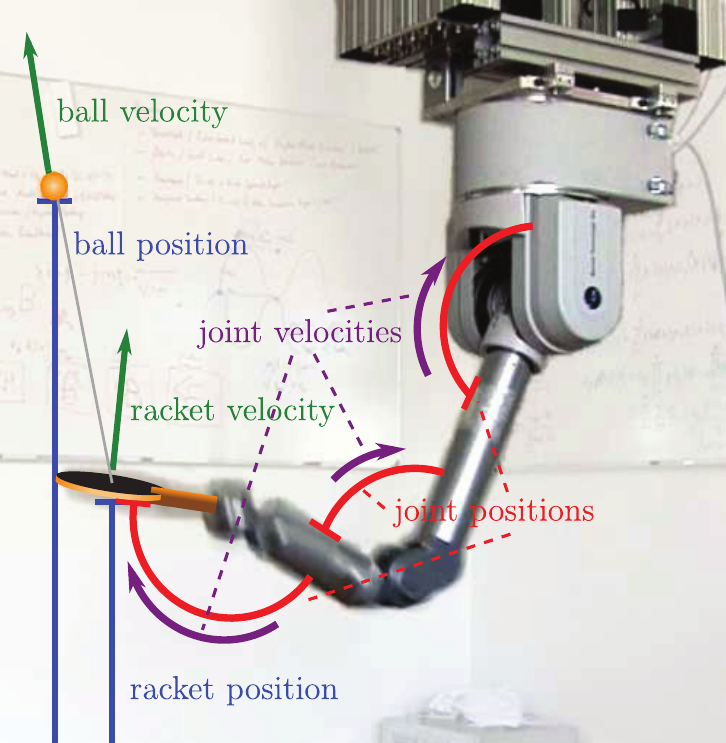
\includegraphics[width=0.3\textwidth]{Images/ball_paddling.png}
    \caption{Ball Paddling Robot}
    \label{fig:ball_paddling_robot}
\end{figure}

This problem is solved with function approximators like neural networks using Deep Reinforcement Learning algorithms.

\subsubsection{Curse of real-world samples}
Robots interact with the physical world, hence robot reinforcement learning suffers from most of the resulting real-world problems.
For example, robot hardware is usually expensive, suffers from wear and tear, and requires careful maintenance. This is why safe exploration
becomes a key issue in the learning process.

Several more aspects of the real-world make robotics a challenging domain. Frequently, the environment settings during an earlier 
learning period cannot be reproduced. This problem makes comparing algorithms particularly hard. Furthermore, the approaches often have to deal 
with uncertainty due to inherent measurement noise and the inability to observe all states directly with sensors.

Most real robot learning tasks require some form of human supervision, e.g. putting the pole back on the robot's end-effector during pole balancing
 after a failure. Even when an automatic reset exists, the learning speed becomes essential as a task on a real robot cannot be sped up.
In some tasks such as a slowly rolling robot, the dynamics can be ignored; in others such as a flying robot, they cannot. In particular in the latter case,
often the whole episode needs to be completed as it is not possible to start from arbitrary states.

For such reasons, real-world samples are expensive in terms of time, labor and, potentially, finances. In robotic reinforcement learning,
it is often considered to be more important to limit the real-world interaction time instead of limiting memory consumption or computational complexity.
Thus, sample efficient algorithms that are able to learn from a small number of trials are essential.

Since the robot is a physical system, there are strict constraints on the interaction between the learning algorithm
and the robot setup. For dynamic tasks, the movement cannot be paused and actions must be selected within a time-budget without 
the opportunity to pause to think, learn or plan between actions.

As reinforcement learning algorithms are inherently implemented on a digital computer, the discretization of
time is unavoidable despite that physical systems are inherently continuous time systems. Time-discretization of the
actuation can generate undesirable artifacts (e.g. the distortion of distance between states) even for idealized physical
systems, which cannot be avoided. As most robots are controlled at fixed sampling frequencies (in the range between
500 Hz and 3 kHz) determined by the manufacturer of the robot, the upper bound on the rate of temporal discretization
is usually pre-determined. The lower bound depends on the horizon of the problem, the achievable speed of changes in
the state, as well as delays in sensing and actuation. All physical systems exhibit such delays in sensing and
actuation. The state of the setup (represented by the filtered sensor signals) may frequently lag behind the real state due
to processing and communication delays. More critically, there are also communication delays in actuation as well
as delays due to the fact that neither motors, gear boxes nor the body's movement can change instantly. Owing to
these delays, actions may not have instantaneous effects but are observable only several time steps later. In contrast, 
in most general reinforcement learning algorithms, the actions are assumed to take effect instantaneously as such
delays would violate the usual Markov assumption. This effect can be addressed by putting some number of recent
actions into the state. However, this significantly increases the dimensionality of the problem.
The problems related to time budgets and delays can also be avoided by increasing the duration of the time steps.
One downside of this approach is that the robot cannot be controlled as precisely; another is that it may complicate a
description of system dynamics.

\subsubsection{Curse of under-modeling and model uncertainty}
One way to offset the cost of real-world interaction is to use accurate models as simulators. In an ideal setting, this
approach would render it possible to learn the behavior in simulation and subsequently transfer it to the real robot.
Unfortunately, creating a sufficiently accurate model of the robot and its environment is challenging and often requires
very many data samples. As small model errors due to this under-modeling accumulate, the simulated robot can
quickly diverge from the real-world system.

Fot tasks where the system is self-stabilizing (that is, where the robot does not require active control to remain in a safe state or return to it),
transferring policies often works well. Nevertheless, tasks can often be learned better in the real world than in simulation due to complex mechanical interactions
that have proven difficult to model accurately. In contrast, in unstable tasks small variations have drastic consequences. For example, in a pole balancing
task, the equilibrium of the upright pole is very brittle and constant control is required to stabilize the system. Transferred policies often perform poorly
in this setting.

\subsubsection{Curse of goal specification}
In reinforcement learning, the desired behavior is implicitly specified by the reward function. The goal of reinforcement
learning algorithms then is to maximize the accumulated long-term reward. While often dramatically simpler than
specifying the behavior itself, in practice, it can be surprisingly difficult to define a good reward function in robot
reinforcement learning. The learner must observe variance in the reward signal in order to be able to improve a
policy: if the same return is always received, there is no way to determine which policy is better or closer to the
optimum. In many domains, it seems natural to provide rewards only upon task achievement, for example, when a table tennis
robot wins a match. This view results in an apparently simple, binary reward specification. However, a robot may
receive such a reward so rarely that it is unlikely to ever succeed in the lifetime of a real-world system. Instead of
relying on simpler binary rewards, we frequently need to include intermediate rewards in the scalar reward function
to guide the learning process to a reasonable solution, a process known as \textit{reward shaping} \cite{Laud2004}.

\subsubsection{SAC in Robotics}
SAC \cite{SAC} achieves state of the art performance for robotic tasks in simulation and real-world scenarios as it is able to
handle continuous state-action spaces and is an off-policy algorithm.
As described in \cite{SAC_modified}, the authors successfully used SAC to learn policies for a quadrupedal locomotion task and
a dexterous hand manipulation task in real-world. Being an off-policy algorithm SAC is more sample efficient than other on-policy
algorithms like PPO \cite{PPO} and this helps mitigating the curse of real-world samples.

\section{ATACOM}
One important factor that cannot be neglected in real-world applications is the necessity of satisfying constraints.
Many practical considerations can be formulated in the form of constraints, such as safety and mechanical viability. For example,
in the robot manipulation task, the robot should not take actions that damage the environment and cannot take actions that exceed
its feasible range.

In order to achieve safe exploration during learning process in continuous control problems different algorithms have been developed.
This section describes one of them, called ATACOM \cite{Atacom}.
 
ATACOM transforms a constrained RL problem into a typical unconstrained RL problem. Hence the problem can be addressed by any
model-free RL algorithm while maintaining the constraints below the tolerance. Furthermore, ATACOM can handle both equality and inequality
constraints.

The state variable $s \in \mc{S}$ is decomposed in the directly controllable state $q \in \mc{Q}$ and uncontrollable state, i.e., $s = \left[\begin{smallmatrix} \bm{q} & \bm{x}\end{smallmatrix}\right]^\intercal$.
We assume that the constraints $\bm{c}(\bm{q}) \le \bm{0}$ are known and depend purely on the controllable state. 

The idea behind ATACOM is to construct the constraint manifold $\bm{\mc{M}_c} : \bm{c}(\bm{q}) = \bm{0}$, determine the bases $\bm{N_c}$ of the tangent space $\bm{\mc{T}_c}$
and sample state velocity in the tangent space (Figure \ref{fig:constraint_manifold}).

\begin{figure}[H]
    \centering
    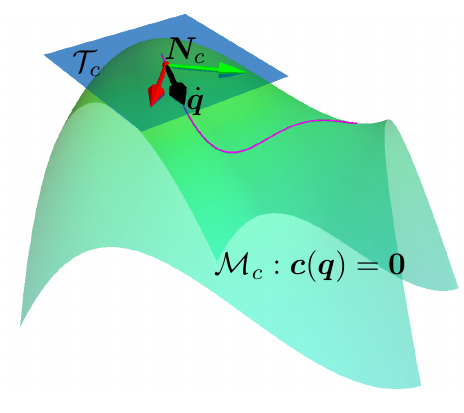
\includegraphics[width=0.3\textwidth]{Images/constraint_manifold.png}
    \caption[ATACOM]{
        Acting on the Tangent Space of the Constraint Manifold. The constraint set $\bm{c}(\bm{q}) = \bm{0}$ is a differentiable manifold
        $\mc{M}_c$ embedded in the original state space. A set of basis $\bm{N}_c$ is used to represent the span of tangent space $\bm{\mc{T}}_c$.
        The tangent space velocity/acceleration can be determined by a coordinate based on the basis, and the control action is determined based on the tangent
        space velocity/acceleration, the resulting trajectory is maintained on the constraint manifold.
        }
    \label{fig:constraint_manifold}
\end{figure}

% The state constraints are defined as
% \begin{equation}
%     \label{eq:state_constraints}
%     \bm{f}(\bm{q}) = \bm{0},\quad \bm{g}(\bm{q}) \le \bm{0},
% \end{equation}
% where $\bm{f} : \mathbb{R}^Q \to \mathbb{R}^F, \bm{g} : \mathbb{R}^Q \to \mathbb{R}^G$ are two $C^2$ mappings for $F$ equality and $G$ inequality
% constraints, and $F < q$. We add the slack variable $\bm{\mu} \in \mathbb{R}^G$ in inequality constraints to convert the original constraints \eqref{eq:state_constraints}
% into equality constraints

% \begin{equation}
%     \label{eq:state_constraints_2}
%     \bm{c(q,\mu)} =
%     \begin{bmatrix}
%         \bm{f}(\bm{q}) & \bm{g}(\bm{q}) + \frac{1}{2}\bm{\mu}^2
%     \end{bmatrix} = \bm{0}.
% \end{equation}

% The constaints set \eqref{eq:state_constraints_2} is a $(F + G)$ dimensional manifold embedded in $(Q + G)$ dimensional space. We calculate the time derivative
% of \eqref{eq:state_constraints_2}

% \begin{equation}
%     \bm{\dot{c}}(\bm{q},\bm{\mu},\bm{\dot{q}},\bm{\dot{\mu}}) = 
%     \begin{bmatrix}
%         \bm{J_f}(\bm{q}) & \bm{0} \\
%         \bm{J_g}(\bm{q}) & diag(\bm{\mu})
%     \end{bmatrix}
%     \begin{bmatrix}
%         \bm{\dot{q}} \\
%         \bm{\dot{\mu}}
%     \end{bmatrix}
%     = \bm{J_c}(\bm{q},\bm{\mu})
%     \begin{bmatrix}
%         \bm{\dot{q}} \\
%         \bm{\dot{\mu}}
%     \end{bmatrix},
% \end{equation}

% with the jacobians $\bm{J_f} \in \mathbb{R}^{F \times Q}$ and $\bm{J_g} \in \mathbb{R}^{G \times Q}$ of $\bm{f}(\bm{q})$ and $\bm{g}(\bm{q})$, respectively.
% Both Jacobians are combined into the Jacobian Matrix $\bm{J_c}(\bm{q}, \bm{\mu}) \in \mathbb{R}^{(F+G) \times (Q + G)}$ of the complete constraint set.

% We can find the null space matrix $\bm{N_c}(\bm{q}, \bm{\mu}) = Null\left[\bm{J_c}(\bm{q},\bm{\mu})\right] \in \mathbb{R}^{(Q+G)\times(Q-F)}$ via SVD.


The advantages of ATACOM can be summarized as follows:
\begin{itemize}
    \item It can deal both with \textbf{equality and inequality constraints}. All of the constraints at each time step are maintained
    below the tolerance during the whole process.
    \item It does not require an initial feasible policy, the agent can \textbf{learn from scratch}.
    \item It requires \textbf{no manual safe backup policy} to move the system back into the safe region.
    \item It can be applied to any model-free RL algorithm, using both \textbf{deterministic and stochastic policies}
    \item It can focus the exploration on the \textbf{lower-dimensional manifold} instead of exploring in the original action space
    for equality constrained problem.
    \item It has \textbf{better learning performance} as the inequality constraints restrict to a smaller feasible state-action space.
\end {itemize}

As a downside this method requires
\begin{itemize}
    \item differentiable constraint functions.
    \item a sufficiently accurate invertible dynamics model of the robot or a well-performed tracking controller.
\end{itemize}

% \begin{definition}
%     A Constrained Markov Decision Process (CMDP) is a tuple $(\mc{S}, \mc{A}, P, R, \gamma, \mc{C})$, where $\mc{S}$ is a state-space,
%     $\mc{A}$ is an action space, $P: \mc{S}\times\mc{A}\times\mc{S} \to [0,1]$ is a transition kernel, $\gamma$ is a discount factor,
%     and $\mc{C}: \left{c_i : \mc{S} \to \mathbb{R} | i \in 1, \dots, k}$ is a set of \textit{immediate state-constraint} functions.
% \end{definition}


\section{Hierarchical Reinforcement Learning}
When tasks are too complex, it is often easier to decompose it into more manageable sub-tasks. Hierarchical Reinforcement Learning
is a learning paradigm that aims to achieve this using temporal abstraction:

Reasoning on multiple time scales using temporally extended actions (sub-behaviors) that consist of a sequence of primitive actions
and possibly other temporally extended actions.

The following information is derived from \cite{survey_mdpi}.

\subsection{Options Framework}
Here, a popular framework to achieve temporal abstraction in reinforcement learning, the \textit{option framework} \cite{Options}, is described.

\begin{definition}
    An Option is a tuple $\omega = (I, \pi, \beta)$ where
    \begin{itemize}
        \item $I \in \mc{S}$ is the initiation set, which defines the states in which the option can be initiated
        \item $\beta: \mc{S} \rightarrow [0, 1]$ is the termination condition that decides when an option will halt its execution
        \item $\pi: \mc{S} \times \mc{A} \rightarrow [0,1]$ is the intra-option policy.
    \end{itemize}
\end{definition}

A policy-over-options $\pi(\omega|s_t)$ selects an option $\omega \in \Omega$ given a state $s_t$. This additional policy can be useful
to select the best options, when the current state belongs to multiple option initiation sets. It can also be used as an alternative to defining
an initiation set for each option.

The most often used execution model is the call-and-return model. This approach is often also called hierarchical-execution.
In this model a policy-over-options selects an option according to the current state. The agent follows this option until the 
agent triggers the termination condition of the active option.

\begin{figure}[b]
    \centering
    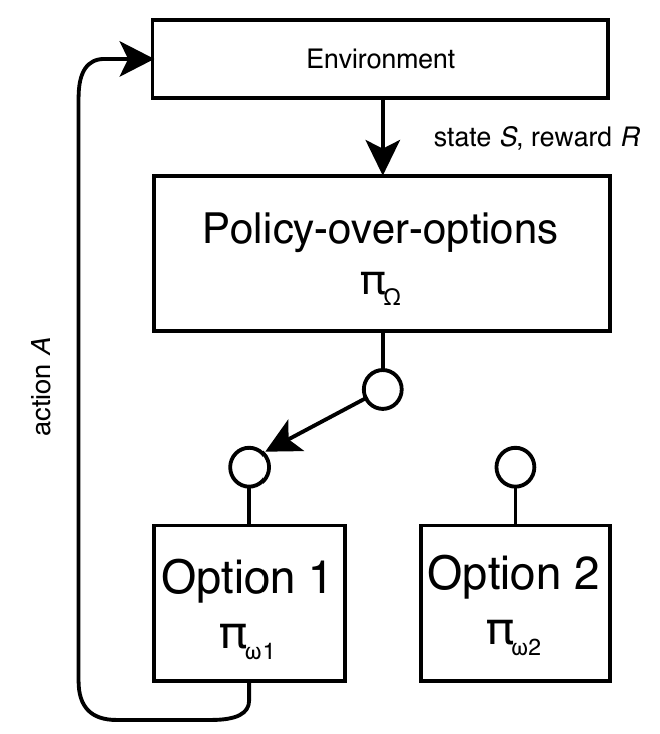
\includegraphics[width=0.3\textwidth]{Images/options_framework.png}
    \caption{Options framework}
    \label{fig:options_framework}
\end{figure}

Motion templates \cite{motion_templates} are options that can be parameterized in order to adapt the behavior of its intra-option policy.
This is often useful in a continuous state-space. A motion template could for example be discovered for throwing a ball, The exhibited
force and angle might be parameters of this template. Learning a single policy for each possible combination of force-angle would be infeasible.

\subsubsection{Option-Critic Framework}

The task of learning options can be decoupled from learning the policy-over-options. The agent can focus first on finding useful temporal
abstractions that simplify the environment. However this approach of bottom-up learning risks wasting time learning sub-behaviors which might not be required
in order to solve the problem at hand. Formulating options development and discovery as part of an optimization problem tasked with optimizing
total future reward is an alternative approach which allows options and a policy-over-options to be learned end-to-end.

The Option-Critic architecture (OC) \cite{option-critic} is an end-to-end framework capable of discovering and developing options without
using prior knowledge. The actor part in the OC framework consists of multiple intra-options policies. The critic part is capable of assessing discounted
future value of options and actions.

PPOC \cite{PPOC} extends the Option-Critic algorithm for continuous control tasks using PPO \cite{PPO}, a popular on-policy deep reinforcement learning algorithm.

\begin{figure}[H]
    \centering
    \label{fig:options_critic}
    \caption{Option-Critic Architecture.}
    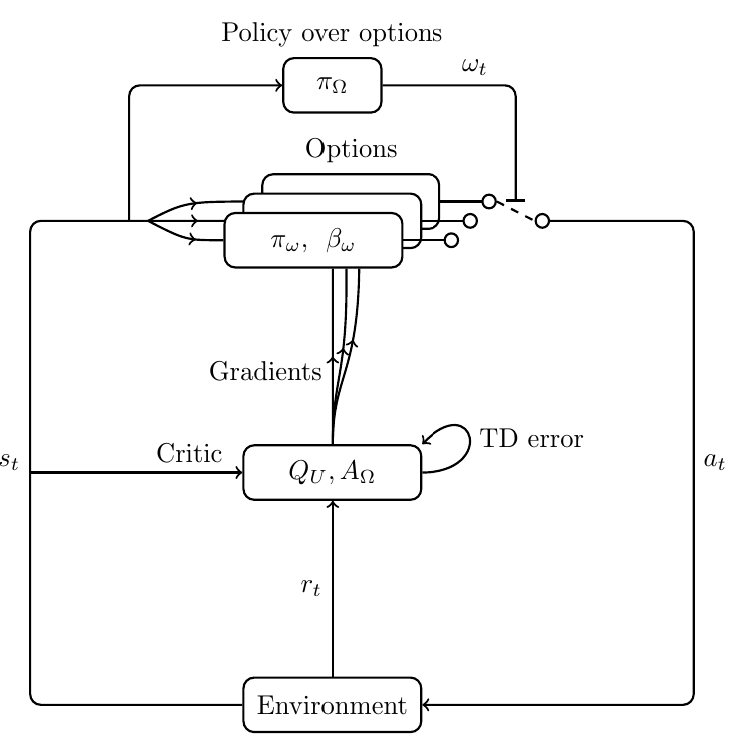
\includegraphics[scale=0.2]{Images/option-critic.png}
\end{figure}

\subsection{Goal-Conditional Framework}

Options are difficult to scale to support numerous sub-behaviors. Training options is inefficient because most commonly only
one option is trained at the time and no components are shared between them.

Here a different approach is presented, the goal-conditional framework.

The goal-conditional framework models sub-behaviors differently. In order to support a large amount of sub-behaviors
a goal-vector $z \in Z$ is utilized to express different sub-behaviors.
The goal-vector characterizes the desired sub-behavior activated by a higher-level manager to a lower-level worker.
The idea is illustrated in Figure \ref{fig:goal-conditional}. This goal-vector can be discrete in order to express
a limited number of abstractions, but it is also possible to use a continuous vector to express an infinite number of possible abstractions.


\begin{figure}
    \centering
    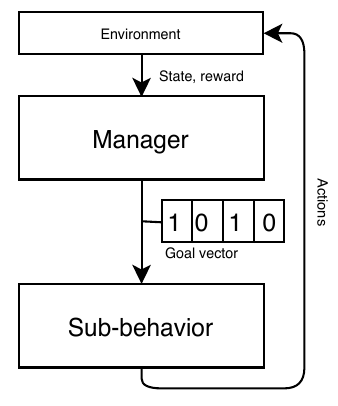
\includegraphics[width=0.3\textwidth]{Images/goal-conditional.png}
    \caption{Goal-Conditional framework.}
    \label{fig:goal-conditional}
\end{figure}

Here are two particular approaches used in the goal-conditional framework:

\begin{itemize}
    \item General Value Function (GVF)
    \item Information Hiding
\end{itemize}

In the \textbf{General Value Function} \cite{Horde} approach different prediction targets are used besides the extrinsic reward signal.
Examples of such targets are, learning how many steps there are
before an episodic control problem terminates, or learning the distance before hitting a wall.
Learning different value functions, can be seen as a way to build general knowledge about
how different aspects of the environment can be manipulated. The intuition behind this
idea is that if we know how our environment works, we should be able to easier achieve
goals in this environment. Different value functions can essentially be utilized as temporal
abstractions, allowing the agent to reason on a higher level of abstraction.
The Horde algorithm \cite{Horde} is capable of learning different targets using independent sub-agents called demons.
Similarly, the Universal Value Function Approximator (UVFA) learns a single value function $V(s, z)$ where the goal-state $z$ is a parameter.
UVFA has also been demonstrated to work in a RL setting, by using Horde.

In the \textbf{Information Hiding} \cite{Feudal_rl} approach no single part of the architecture has access to all available information and different parameters
need to collaborate. While the GVF framework focuses on decomposing the reward function, information hiding focuses on decomposing the state-space.


Algorithms such as HIRO \cite{HIRO} are capable of learning diverse sets of sub-behaviors and their composition, end-to-end, in function
of the extrinsic reward. The HIRO architecture, illustrated in Figure \ref{fig:HIRO}.
In HIRO, the higher level communicates directional subgoals. These subgoals are represented using the state-space and the
lower level is densely rewarded for moving towards this subgoal-state. Other end-to-end algorithms such as FeUdal Networks \cite{FuN}
use a low dimensional latent space to represent sub-behaviors.
The HIRO approach focuses on sample efficiency by supporting off-policy learning. Off-policy corrections are used to
make up for the combinatorial effects introduced by simultaneously learning a lower-level policy and a higher-level policy.
This correction re-labels past experience with a high-level action, in order to maximize the probability of the past lower-level actions.

\begin{figure}
    \centering
    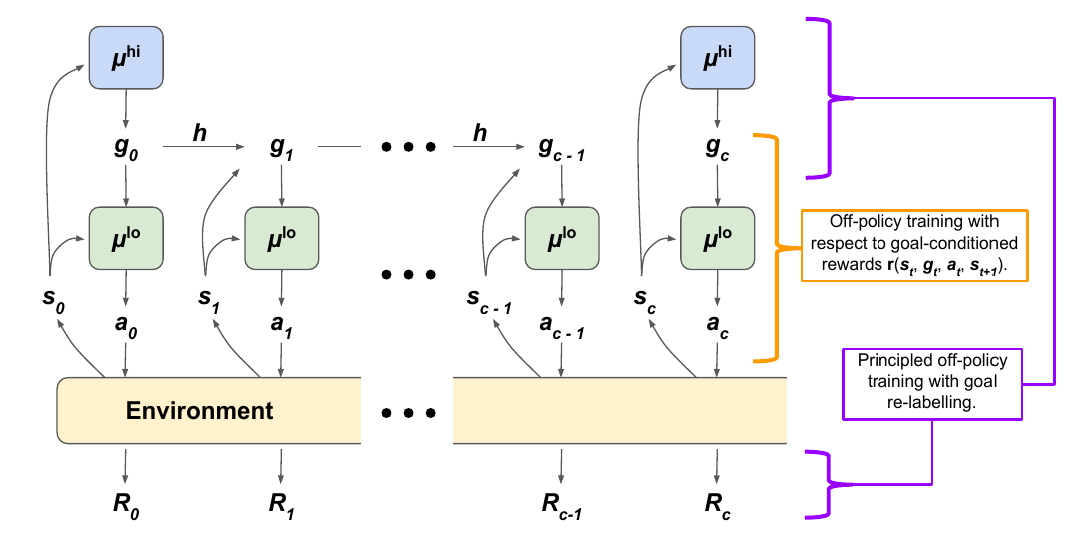
\includegraphics[width=0.8\textwidth]{Images/HIRO.png}
    \caption{HIRO architecture.}
    \label{fig:HIRO}
\end{figure}


\chapter{Robot Air Hockey Challenge}
\label{ch:robot_air_hockey_challenge}
This chapter describes the Robot Air Hockey completition that took place from 20 February 2023 to 1 November 2023.
It covers the game rules, the motivation behind the event, the various stages of the competition and the outcomes achieved.
The following information is derived from the challenge's website, i.e., \url{https://air-hockey-challenge.robot-learning.net}.

\subsection{Air Hockey Game}
Air Hockey is a zero sum game in which two opponents compete interacting with a puck on a table and trying to score a goal
sending the puck into the opponent's goal while at the same time preventing the opponent from scoring.
The table is rectangular and smooth, with low-friction achieved by air blown from under the surface, designed to mimic the surface of ice.
This game is dynamic and the puck reaches high velocities that require the players to have quick reflexes and strategic positioning.

For this competition the players are robotic manipulators

\subsection{Motivation}
This competition was organized to \textit{close the sim-to-real gap}, i.e., the differences and challenges that arise
when transferring a robotic system trained in a simulated environment to the real world.
In fact, when transferring the robotic system to the real world we have to deal with
\begin{itemize}
    \item disturbances
    \item observation noise
    \item safety
    \item model mismatch
    \item delays
    \item actuator limitations
    \item physical feasibility
    \item limited real-world interaction
\end{itemize}

The Robot Air Hockey Challenge provides a platform for researchers in the field of robot learning to interact with each
other on a realistic robotic task. In this competition team had to design and build their air hockey agents, competing against
each other in different subtasks (in simulation) and finally in an entire game (both in simulation and in the real world).

\section{Challenge organization}
\label{sec:organization}
The challenge consists in three simulated stages: Warm Up, Qualifying and Tournament. Each stage consists of different tasks
required for robot air hockey. Apart from executing the given tasks the robots needs to be robust and capable of adapting to changes.
Except from the Warm Up stage the submitted agents are evaluated in modified simulation environments to mimic the sim-to-real gap.

The first three teams are able to deploy their approach on the real robot and compete in a real world scenario.

\subsection{Warm-Up Stage}
In the Warm-Up stage the participants were given an ideal environment with a 3-degree-of-freedom robot. This stage aimed to familiarize with the given tasks,
the environment and the application programming interface.

The tasks given at this point were two:
\begin{itemize}
    \item \textbf{Hit}: The puck is randomly initialized on the left side of the table. The initial velocity is zero. The objective is to hit the puck
    to score a goal as fast as possible.
    \item \textbf{Defend}: The puck is randomly initialized on the right side of the table with a random velocity heading left.
    The objective is to stop the puck on the right side of the table and prevent it from getting scored.
\end{itemize}
\subsection{Qualifying Stage}
\label{subsec:qualifying_stage}
In this stage the participants were given an environment exposing an interface to control a general-purpose robot, the KUKA-iiwa14 LBR.
At this point the submitted agents to the challenge's cloud evaluator were simulated with a modified version of the environment handed to the participant teams
in order to simulate different types of real world problems. This modifications included disturbances, observation noise, loss of tracking, model mismatch, and imperfect trakcing controller.

Each team could evaluate its solution once per task per day. Each evaluation was conducted with 1000 episodes, equivalently 2.8 hours of real-world experiments.
Based on the evaluation metric, the agents were categorized into three levels:
\begin{itemize}
    \item Deployable
    \item Improvable
    \item Nondeployable.
\end{itemize}

The given tasks at this stage were three:

\begin{itemize}
    \item \textbf{Hit}: The opponent moves in a predictable pattern. The puck is randomly initialized with a small velocity. The objective is to score the goal as many times as possible.
    The episode ends when the puck is scored or it bounces back. The episodes terminates with \textit{success} if the puck is scored.
    \item \textbf{Defend}: The puck is randomly initialized on the right side of the table with a random velocity heading left.
    The objective is to stop the puck on the right side of the table and prevent it from getting scored.
    The episode terminates if the puck is returned to the opponent's side or scored or the puck speed dropbs below the threshold.
    The episode terminates with \textit{success} if the puck is in the range where hits can be made and the longitudinal speed is below the threshold.
    \item \textbf{Prepare}: The puck is initialized close to the table's boundary and is unsuitable for hitting. The task is to control the puck to move it into a good hit position. The puck is not allowed to cross the middle line.
    The episodes terminates if the puck crosses the middle line that connects the middle points of two goals, or the puck is on the opponent's side of the table.
    The episodes terminates with success if the puck is in the range where its can be made and the longitudinal speed is below the threshold.
\end{itemize}

\subsection{Tournament Stage}
Only the participant teams who submitted agents that were categorized as Deployable or Improvable were qualified to participate in the tournament stage.
The maximum number of teams is 16, which were determined based on the ranking of \textit{success rate} in the qualifying stage.
In this stage each team had to develop an agent able to play the whole game.
A hard coded baseline based on the implementation in \cite{baseline} agent was provided to test and validate the agents before the actual competition started. 

The tournament stage was divided into two rounds. After the first rounds teams had two weeks to adjust and improve their agent.
Teams were awarded three points if they won a match, otherwise one point if they drew and zero if they lost.
The final ranking of the tournament was determined by the total score of the two rounds.

\subsubsection{Game Rules}
\begin{itemize}
    \item A game is 15 minutes in length, i.e. 45000 steps.
    \item The first player to accumulate seven (7) points wins the game. If no player accumulates seven points within the designated competition time, the player with the most points wins.
    \item To score a point, the puck must fully enter the goal. Rebounds or pucks that get stuck halfway in do not count as a point.
    \item When a player makes a goal, the other player serves the puck next.
    \item A player may only strike the puck when it is on their side of the centerline.
    \item Mallets may not cross the center line when striking the puck.
    \item When the puck stops in the middle of the table (20cm width), the puck is reset randomly to one player's side
    \item “Topping” the puck is not allowed. This means players cannot lift their mallet and place it over the puck to hold it in place.
    \item Touching the puck with other parts of the robot is not allowed.
    \item Once the puck is on a certain player's side of the center line, the player has 15 seconds, i.e. 750 steps, to hit the puck back across the center line. Otherwise a foul is committed and the opponent receives possession of the puck.
\end{itemize}

\section{Framework}
The Air Hockey Challenge is built upon MushroomRL \cite{mushroom_rl}, a Reinforcement Learning Library.
The general framework of challenge consists of two key components, i.e., \textit{Agent} and \textit{AirHockeyChallengeWrapper}.
A schema of the framework can be seen in Figure \ref{fig:framework}.
Participants had to implement the \textit{Agent} component.

\begin{figure}[H]
    \centering
    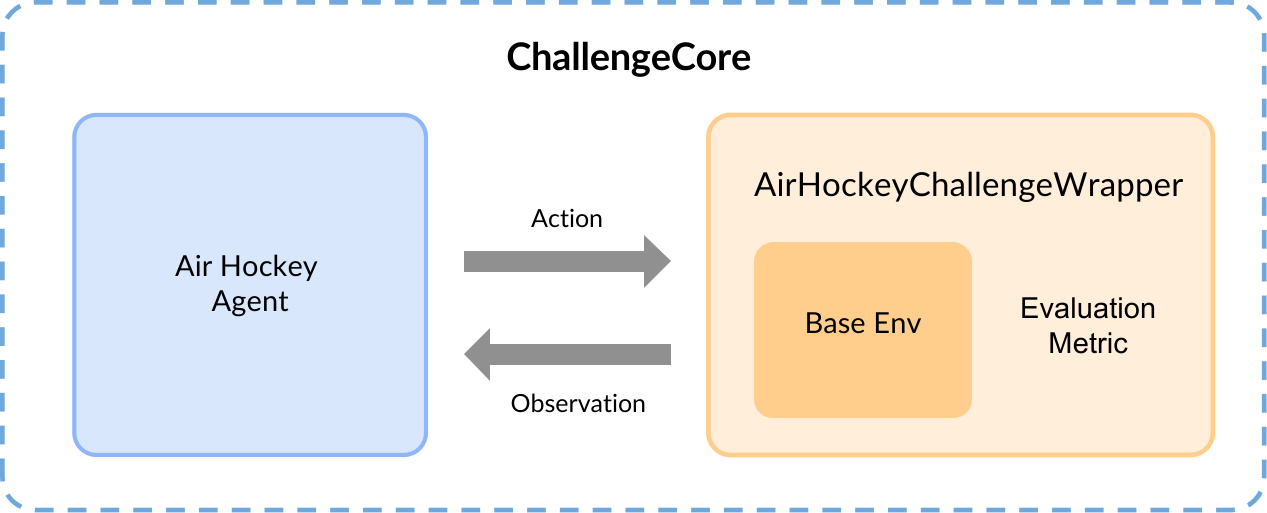
\includegraphics[width=0.8\textwidth]{Images/framework.png}
    \caption{Challenge framework.}
    \label{fig:framework}
\end{figure}

\subsection{Environments}
    The \textit{AirHockeyChallengeWrapper} component is a wrapper for the \textit{Base env} and processes the necessary information for the challenge evaluation.

    The simulated environment tries to mimic the real-world setup. The robot is controlled by a \textit{Tracking controller}, a Feedforward-PD controller, which sends 
    the torque command $\tau_{cmd}$ to the robot.

    \begin{equation*}
        \tau_{cmd} = M(q)\ddot{q}_d + c(q,\dot{q}) + g(q) + K_p(q_d - q) + K_d(\dot{q}_d - \dot{q})
    \end{equation*}

    The \textit{Trajectory interpolator}, by default a cubic polynomial, is used to interpolate the trajectory points between two consecutive commands.
    A \textit{Joint safety limiter} is used to avoid executing commands that exceed the position or velocity limits.

    \begin{figure}[H]
        \centering
        \label{fig:control_loop}
        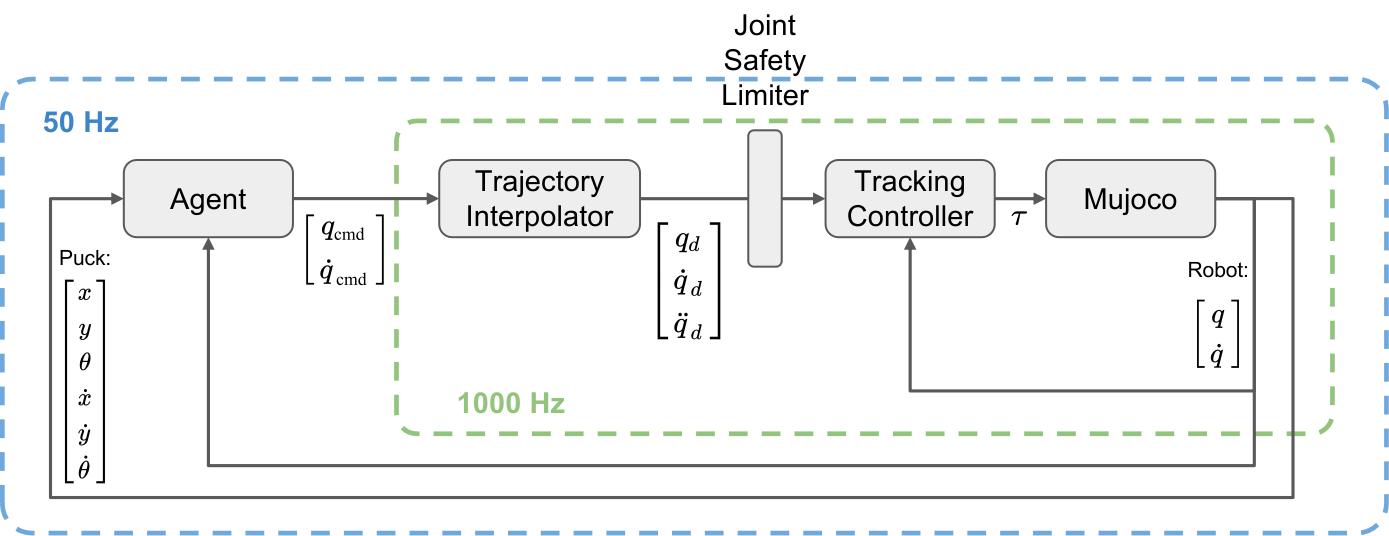
\includegraphics[width=0.8\textwidth]{Images/control_paradigm}
        \caption{Control loop.}

    \end{figure}

    %% Interpolation options

    The framework provides a flexible interface for commanding the robot in which the trajectory interpolation order can be specified:
    \begin{itemize}
        \item Cubic interpolation. The action command contains the desired [position, velocity]. A cubic polynomial is used to interpolate the intermediate steps.
        \item Linear interpolation. The action command contains the desired [position]. A linear polynomial is used to interpolate the intermediate steps.
        \item Quadratic interpolation. The action command contains the desired [position]. A quadratic function uses the previous position, velocity and the desired position to interpolate the intermediate steps.
        \item Quartic interpolation. The action command contains the desired [position, velocity]. A quartic function uses the previous position, velocity and the desired position, velocity to interpolate the intermediate steps.
        \item Quintic interpolation. The action command contains the desired [position, velocity, acceleration]. A quintic function is computed by the previous position, velocity, acceleration and the desired position, velocity and acceleration to interpolate the intermediate steps.
        \item Linear interpolation in position and velocity. The action command contains the desired [position, velocity]. The position and velocity will both be linearly interpolated. The acceleration is computed based on the derivative of the velocity. This interpolation is not proper, but it is useful to avoid oscillatory in the interpolation.
        \item None. The action can be a complete trajectory between each action step. At each step, the trajectory command should include desired [position, velocity, acceleration]
    \end{itemize}

    The air hockey table and its dimensions are illustrated in Figure \ref{fig:air_hockey_table}


    \begin{figure}[H]
        \centering
        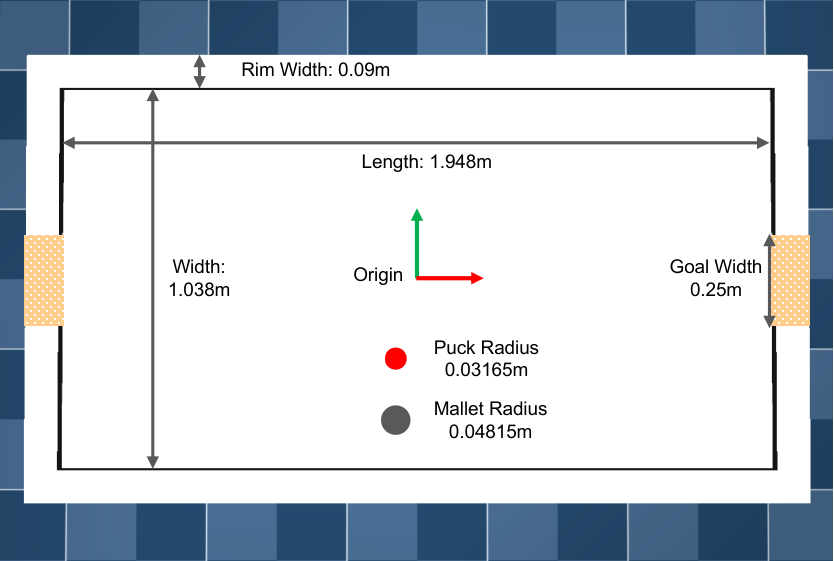
\includegraphics[width=0.8\textwidth]{Images/air_hockey_table}
        \caption{The air hockey table.}
        \label{fig:air_hockey_table}
    \end{figure}

\subsection{Robot models}
    \subsubsection{Planar robot - 3 degrees of freedom}
    During the Warm up stage the participants were provided a 3 DoF planar robot to understand how to use the framework.
    The robot is set such that the end-effector remains at the same height of the table surface. In simulation, the collision between the robot and the table are discarded.
    The base of the planar robot is located at [-1.51, 0., -0.1], the orientation is aligned with the world's frame, as illustrated in Figure \ref{fig:planar_env}


    Below the specification of the planar robot:
    \begin{itemize}
        \item \textbf{Position upper limit (rad)}: [ 2.967060, 1.8, 2.094395]
        \item \textbf{Position lower limit (rad)}: [-2.967060, -1.8, -2.094395]
        \item \textbf{Velocity limit (rad/s)}: +/- [1.570796, 1.570796, 2.094395]
        % \item \textbf{Link length (m)}: [0.55, 0.44, 0.44]
        \item \textbf{Initial position (rad)}: [-1.156, 1.300, 1.443]
        \item \textbf{Initial velocity (rad/s)} [0, 0, 0]
    \end{itemize}

    \subsubsection{KUKA iiwa14 LBR robot}
    The KUKA iiwa14 LBR robot is a general purpose manipulator with 7 degrees of freedom. A universal joint on the end-effector is added
    to increase the robot's flexibility. The universal joint is a passive joint that adapts the joint position based on contacts. In simulation, the collision between the robot and the table
    are discarded, requiring the agent to keep the mallet at an appropriate height.

    We define the End-Effector as the tip of the extension rod before the universal joint. 
    The end-effector's position can be fully determined by the robot's joint position and forward kinematics. 
    The base position of the robot is depicted in Figure \ref{fig:kuka_env}.

    Below the specification of the planar robot:
    \begin{itemize}
        \item \textbf{Position upper limit (rad)}: [ 2.967, 2.09 , 2.967, 2.094, 2.967, 2.094, 3.054]
        \item \textbf{Position lower limit (rad)}: [-2.967, -2.094, -2.967, -2.094, -2.967, -2.094, -3.054]
        \item \textbf{Velocity limit (rad/s)}: +/- [ 1.483, 1.483, 1.745, 1.308, 2.268, 2.356, 2.356]   
        \item \textbf{Initial position (rad)}: [ 0, -0.1960, 0, -1.8436, 0, 0.9704 0]
        \item \textbf{Initial velocity (rad/s)} [0, 0, 0, 0, 0, 0, 0]
    \end{itemize}


\subsection{Constraints}
To avoid losing points the robot must respect a set of constraints.
These constraints are described here:

\begin{itemize}
    \item \textit{JointPositionConstraint}: $q_l < q_{cmd} < q_u$
    \item \textit{JointVelocityConstraint}: $\dot{q}_l < \dot{q}_{cmd} < \dot{q}_u$
    \item \textit{EndEffectorConstraint}:
        \begin{equation*}
            \begin{aligned}
                & l_x < x_{ee} \\
                & l_y < y_{ee} < u_y \\
                & \text{table height} - \text{tolerance} < z_{ee} < \text{table height} + \text{tolerance}
            \end{aligned}
        \end{equation*}
    The End-Effector must not exceed the table and stay at
    \item \textit{LinkConstraint} (7 DoF Robot only):
    \begin{equation*}
        \begin{aligned}
            & z_{elbow} > 0.25 \\
            & z_{wrist} > 0.25
        \end{aligned}
    \end{equation*}
    \item \textit{ComputationTime}: The computation time at each step should be smaller than 0.02s.
\end{itemize}

\subsection{Evaluation Metrics}
    \begin{itemize}
        \item \textbf{Success Rate}:
        A success criterion is defined for each task. We will check if the task succeed when the episode terminates. Each episode can terminate because of two reasons: 1. maximum number of steps reached; 2. No further interaction can be in the episodes.
        \begin{itemize}
            \item Hit: The puck enters the scoring zone with a speed above the threshold.
            \item Defend: The final velocity of the puck (at the end of the game) is below the threshold and does not bounce to the other side of the court.
            \item Prepare: The final position of the puck is within a predefined area and at a speed less than the threshold.
        \end{itemize}

        \item \textbf{Deployability}: Each deployability metric is assigned one or multiple penalty points based on the level of risk. The deployability score is counted when the constraints of the evaluation metric are violated. Each metric is computed at most once per episode (maximum 500 steps per episode). 
        \begin{itemize}
            \item Violations of the End-Effector's Position Constraints (3 penalty points): 
            The desired x-y-position of the end-effector should remain within the boundaries of the table. The z-position of the end-effector should remain within a range.
            \item Violations of the Joint Position Limit Constraints (2 penalty points): The desired position command should not exceed the position limits.
            \item Violations of the Joint Velocity Limit Constraints (1 penalty point): The desired velocity command should not exceed the velocity limits.
            \item Computation Time (0.5-2 penalty points): The computation time at each step should be shorter than 0.02s.
        \end{itemize}
    \end{itemize}

    Each evaluation consisted of 1000 episodes. The success rates were used to rank the leaderboards. The deployability score is the sum of the penalty score from all episodes. The rankings were divided into three categories based on the score of deployability.
    \begin{enumerate}
        \item \textbf{Deployable}: $0 \le \text{deployability score} \le 500$
        \item \textbf{Improvable}: $500 < \text{deployability score} \le 1500$
        \item \textbf{Nondeployable}: $1500 < \text{deployability score}$
    \end{enumerate}

\subsection{Simulator}
    The simulator application of the Robot Air Hockey Challenge is summarized in the following:
    \begin{itemize}
        \item Simulator: MuJoCo \cite{MuJoCo}
        \item Simulation frequency: 1000 Hz
        \item Control Frequency: 50 Hz
        \item Observation:
            \begin{itemize}
                \item \textbf{Robot}:
                \begin{itemize}
                    \item Joint positions [radians]
                    \item Joint velocities [radians/s] computed by finite difference
                \end{itemize}
                \item \textbf{Puck} (relative to the robot base frame):
                    \begin{itemize}
                        \item X-Y position [m]
                        \item Yaw angle [radians]
                        \item X-Y velocity [m/s]
                        \item Yaw velocity [radians/s] computed by finite difference
                    \end{itemize}
                \item \textbf{Opponent} (if applicable)
                \begin{itemize}
                    \item End-effector-s X-Y position [m]
                \end{itemize}
            \end{itemize}
        \item Control action:
            \begin{itemize}
                \item We try to set the simulation as close as possible to the real-world setup. The robot is controlled by torque at 1000 Hz. We use a feed-forward + PD controller to determine the joint torque that tracks the desired joint position and velocity.
                \item A 20-step interpolation is required in the agent's adjacent control commands (the agent control frequency is 50 Hz). We provide different types of polynomial interpolation upon requirements. Details about the action interface can be found here.
            \end{itemize}
    \end{itemize}


% \chapter{Chapter one}
\label{ch:chapter_one}%
% The \label{...}% enables to remove the small indentation that is generated, always leave the % symbol.

In this chapter additional useful information are reported.

\section{Sections and subsections}
\label{sec:section_name}
Chapters are typically subdivided into sections and subsections, and, optionally,
subsubsections, paragraphs and subparagraphs.
All can have a title, but only sections and subsections are numbered.
A new section is created by the command
\begin{verbatim}
\section{Title of the section}
\end{verbatim}
The numbering can be turned off by using \verb|\section*{}|.
\\
A new subsection is created by the command
\begin{verbatim}
\subsection{Title of the subsection}
\end{verbatim}
and, similarly, the numbering can be turned off by adding an asterisk as follows 
\begin{verbatim}
\subsection*{}
\end{verbatim}

\section{Equations}
\label{sec:eqs}
This section gives some examples of writing mathematical equations in your thesis.

Maxwell's equations read:
\begin{subequations}
    \label{eq:maxwell}
    \begin{align}[left=\empheqlbrace]
    \nabla\cdot \bm{D} & = \rho, \label{eq:maxwell1} \\
    \nabla \times \bm{E} +  \frac{\partial \bm{B}}{\partial t} & = \bm{0}, \label{eq:maxwell2} \\
    \nabla\cdot \bm{B} & = 0, \label{eq:maxwell3} \\
    \nabla \times \bm{H} - \frac{\partial \bm{D}}{\partial t} &= \bm{J}. \label{eq:maxwell4}
    \end{align}
\end{subequations}

Equation~\eqref{eq:maxwell} is automatically labeled by \texttt{cleveref},
as well as Equation~\eqref{eq:maxwell1} and Equation~\eqref{eq:maxwell3}.
Thanks to the \verb|cleveref| package, there is no need to use \verb|\eqref|.
Remember that Equations have to be numbered only if they are referenced in the text.

Equations~\eqref{eq:maxwell_multilabels1}, \eqref{eq:maxwell_multilabels2}, \eqref{eq:maxwell_multilabels3}, and \eqref{eq:maxwell_multilabels4} show again Maxwell's equations without brace:
\begin{align}
    \nabla\cdot \bm{D} & = \rho, \label{eq:maxwell_multilabels1} \\
    \nabla \times \bm{E} +  \frac{\partial \bm{B}}{\partial t} &= \bm{0}, \label{eq:maxwell_multilabels2} \\
    \nabla\cdot \bm{B} & = 0, \label{eq:maxwell_multilabels3} \\
    \nabla \times \bm{H} - \frac{\partial \bm{D}}{\partial t} &= \bm{J} \label{eq:maxwell_multilabels4}.
\end{align}

Equation~\eqref{eq:maxwell_singlelabel} is the same as before,
but with just one label:
\begin{equation}
    \label{eq:maxwell_singlelabel}
    \left\{
    \begin{aligned}
    \nabla\cdot \bm{D} & = \rho, \\
    \nabla \times \bm{E} +  \frac{\partial \bm{B}}{\partial t} &= \bm{0},\\
    \nabla\cdot \bm{B} & = 0, \\
    \nabla \times \bm{H} - \frac{\partial \bm{D}}{\partial t} &= \bm{J}.
    \end{aligned}
    \right.
\end{equation}

\section{Figures, Tables and Algorithms}
Figures, Tables and Algorithms have to contain a Caption that describe their content, and have to be properly reffered in the text.

\subsection{Figures}
\label{subsec:figures}

For including pictures in your text you can use \texttt{TikZ} for high-quality hand-made figures,
or just include them as usual with the command
\begin{verbatim}
\includegraphics[options]{filename.xxx}
\end{verbatim}
Here xxx is the correct format, e.g. \verb|.png|, \verb|.jpg|, \verb|.eps|, \dots.

\begin{figure}[H]
    \centering
    
\includegraphics[width=0.3\textwidth]{logo_polimi_scritta.eps}
    \caption{Caption of the Figure to appear in the List of Figures.}
    \label{fig:quadtree}
\end{figure}

Thanks to the \texttt{\textbackslash subfloat} command, a single figure, such as Figure~\ref{fig:quadtree},
can contain multiple sub-figures with their own caption and label, e.g. \color{black} Figure~\ref{fig:polimi_logo1} and Figure~\ref{fig:polimi_logo2}. 

\begin{figure}[H]
    \centering
    \subfloat[One PoliMi logo.\label{fig:polimi_logo1}]{
        
\includegraphics[scale=0.5]{Images/logo_polimi_scritta.eps}
    }
    \quad
    \subfloat[Another one PoliMi logo.\label{fig:polimi_logo2}]{
        
\includegraphics[scale=0.5]{Images/logo_polimi_scritta2.eps}
    }
    \caption[Shorter caption]{This is a very long caption you don't want to appear in the List of Figures.}
    \label{fig:quadtree2}
\end{figure}


\subsection{Tables}
\label{subsec:tables}

Within the environments \texttt{table} and  \texttt{tabular} you can create very fancy tables as the one shown in Table~\ref{table:example}.
\begin{table}[H]
    \caption*{\textbf{Title of Table (optional)}}
    \centering 
    \begin{tabular}{|p{3em} c c c |}
    \hline
    \rowcolor{bluepoli!40} % comment this line to remove the color
     & \textbf{column 1} & \textbf{column 2} & \textbf{column 3} \T\B \\
    \hline \hline
    \textbf{row 1} & 1 & 2 & 3 \T\B \\
    \textbf{row 2} & $\alpha$ & $\beta$ & $\gamma$ \T\B\\
    \textbf{row 3} & alpha & beta & gamma \B\\
    \hline
    \end{tabular}
    \\[10pt]
    \caption{Caption of the Table to appear in the List of Tables.}
    \label{table:example}
\end{table}

You can also consider to highlight selected columns or rows in order to make tables more readable.
Moreover, with the use of \texttt{table*} and the option \texttt{bp} it is possible to align them at the bottom of the page. One example is presented in Table~\ref{table:exampleC}. 

\begin{table}[H]
\centering 
    \begin{tabular}{|p{3em} | c | c | c | c | c | c|}
    \hline
%    \rowcolor{bluepoli!40}
     & \textbf{column1} & \textbf{column2} & \textbf{column3} & \textbf{column4} & \textbf{column5} & \textbf{column6} \T\B \\
    \hline \hline
    \textbf{row1} & 1 & 2 & 3 & 4 & 5 & 6 \T\B\\
    \textbf{row2} & a & b & c & d & e & f \T\B\\
    \textbf{row3} & $\alpha$ & $\beta$ & $\gamma$ & $\delta$ & $\phi$ & $\omega$ \T\B\\
    \textbf{row4} & alpha & beta & gamma & delta & phi & omega \B\\
    \hline
    \end{tabular}
    \\[10pt]
    \caption{Highlighting the columns}
    \label{table:exampleC}
\end{table}

\begin{table}[H]
\centering 
    \begin{tabular}{|p{3em} c c c c c c|}
    \hline
%    \rowcolor{bluepoli!40}
     & \textbf{column1} & \textbf{column2} & \textbf{column3} & \textbf{column4} & \textbf{column5} & \textbf{column6} \T\B \\
    \hline \hline
    \textbf{row1} & 1 & 2 & 3 & 4 & 5 & 6 \T\B\\
    \hline
    \textbf{row2} & a & b & c & d & e & f \T\B\\
    \hline
    \textbf{row3} & $\alpha$ & $\beta$ & $\gamma$ & $\delta$ & $\phi$ & $\omega$ \T\B\\
    \hline
    \textbf{row4} & alpha & beta & gamma & delta & phi & omega \B\\
    \hline
    \end{tabular}
    \\[10pt]
    \caption{Highlighting the rows}
    \label{table:exampleR}
\end{table}

\subsection{Algorithms}
\label{subsec:algorithms}

Pseudo-algorithms can be written in \LaTeX{} with the \texttt{algorithm} and \texttt{algorithmic} packages.
An example is shown in Algorithm~\ref{alg:var}.
\begin{algorithm}[H]
    \label{alg:example}
    \caption{Name of the Algorithm}
    \label{alg:var}
    \label{protocol1}
    \begin{algorithmic}[1]
    \STATE Initial instructions
    \FOR{$for-condition$}
    \STATE{Some instructions}
    \IF{$if-condition$}
    \STATE{Some other instructions}
    \ENDIF
    \ENDFOR
    \WHILE{$while-condition$}
    \STATE{Some further instructions}
    \ENDWHILE
    \STATE Final instructions
    \end{algorithmic}
\end{algorithm} 

\vspace{5mm}

\section{Theorems, propositions and lists}

\subsection{Theorems}
Theorems have to be formatted as:
\begin{theorem}
\label{a_theorem}
Write here your theorem. 
\end{theorem}
\textit{Proof.} If useful you can report here the proof.

\subsection{Propositions}
Propositions have to be formatted as:
\begin{proposition}
Write here your proposition.
\end{proposition}

\subsection{Lists}
How to  insert itemized lists:
\begin{itemize}
    \item first item;
    \item second item.
\end{itemize}
How to insert numbered lists:
\begin{enumerate}
    \item first item;
    \item second item.
\end{enumerate}

\section{Use of copyrighted material}

Each student is responsible for obtaining copyright permissions, if necessary, to include published material in the thesis.
This applies typically to third-party material published by someone else.

\section{Plagiarism}

You have to be sure to respect the rules on Copyright and avoid an involuntary plagiarism.
It is allowed to take other persons' ideas only if the author and his original work are clearly mentioned.
As stated in the Code of Ethics and Conduct, Politecnico di Milano \textit{promotes the integrity of research,
condemns manipulation and the infringement of intellectual property}, and gives opportunity to all those
who carry out research activities to have an adequate training on ethical conduct and integrity while doing research.
To be sure to respect the copyright rules, read the guides on Copyright legislation and citation styles available
at:
\begin{verbatim}
https://www.biblio.polimi.it/en/tools/courses-and-tutorials
\end{verbatim}
You can also attend the courses which are periodically organized on "Bibliographic citations and bibliography management".

\section{Bibliography and citations}
Your thesis must contain a suitable Bibliography which lists all the sources consulted on developing the work.
The list of references is placed at the end of the manuscript after the chapter containing the conclusions.
We suggest to use the BibTeX package and save the bibliographic references  in the file \verb|Thesis_bibliography.bib|.
This is indeed a database containing all the information about the references. To cite in your manuscript, use the \verb|\cite{}| command as follows:
\\
\textit{Here is how you cite bibliography entries: \cite{knuth74}, or multiple ones at once: \cite{knuth92,lamport94}}.
\\
The bibliography and list of references are generated automatically by running BibTeX \cite{bibtex}.

\chapter{Conclusions and future developments}
\label{ch:conclusions}%
In this work, reinforcement learning was successfully applied to the air hockey task using a general-purpose manipulator. 
The agent was able to play entire matches without violating too many constraints, thanks to the ATACOM algorithm. 
The SAC method outperformed the rule-based controller for the hitting task, achieving a higher success rate. 
The rule-based switcher effectively selected the appropriate policy at the right time, with its parameters slightly optimized PGPE.

\section{Future works}
The developed rule-based switcher currently uses a few simple parametric rules. 
Future work could involve implementing a more complex switcher with additional rules that also take the opponent's actions into account.

An other strategy could be to apply an end-to-end hierarchical reinforcement learning approach, such as HIRO \cite{HIRO}, where a single low-level policy receives from the high-level
policy a vector to determine the desired behavior.

Since air hockey is a multi-agent setting, investigating a self-play learning strategy could also be beneficial. 
This approach could help the agent improve by continuously adapting to and learning from interactions with itself or other agents.



% %-------------------------------------------------------------------------
%	BIBLIOGRAPHY
%-------------------------------------------------------------------------

\addtocontents{toc}{\vspace{2em}} % Add a gap in the Contents, for aesthetics
\bibliography{Thesis_bibliography} % The references information are stored in the file named "Thesis_bibliography.bib"

%-------------------------------------------------------------------------
%	BIBLIOGRAPHY
%-------------------------------------------------------------------------

\addtocontents{toc}{\vspace{2em}} % Add a gap in the Contents, for aesthetics
\bibliography{Thesis_bibliography} % The references information are stored in the file named "Thesis_bibliography.bib"


%-------------------------------------------------------------------------
%	APPENDICES
%-------------------------------------------------------------------------

\cleardoublepage
\addtocontents{toc}{\vspace{2em}} % Add a gap in the Contents, for aesthetics
\appendix

\chapter{Appendix A}
If you need to include an appendix to support the research in your thesis, you can place it at the end of the manuscript.
An appendix contains supplementary material (figures, tables, data, codes, mathematical proofs, surveys, \dots)
which supplement the main results contained in the previous chapters.

\chapter{Appendix B}
It may be necessary to include another appendix to better organize the presentation of supplementary material.



% LIST OF FIGURES
\listoffigures

% LIST OF TABLES
\listoftables

% LIST OF SYMBOLS
% Write out the List of Symbols in this page
% \chapter*{List of Symbols} % You have to include a chapter for your list of symbols (
% \begin{table}[H]
%     \centering
%     \begin{tabular}{lll}
%         \textbf{Variable} & \textbf{Description} & \textbf{SI unit} \\\hline\\[-9px]
%         $\bm{u}$ & solid displacement & m \\[2px]
%         $\bm{u}_f$ & fluid displacement & m \\[2px]
%     \end{tabular}
% \end{table}

% ACKNOWLEDGEMENTS
% \chapter*{Acknowledgements}
% Here you might want to acknowledge someone.


\cleardoublepage


\end{document}
